\documentclass[10pt, aspectratio=169]{beamer}
\usepackage{docmute}
\usepackage{beamer_theme_408}

\title{408考研零基础 --- 计算机网络}
\author{}
\date{}

\begin{document}

\frame{\titlepage}

\begin{frame}{模块4 计算机网络}
    \begin{columns}[T]
        \column{0.55\textwidth}
        \textbf{本模块包含以下 14 节内容：}
        \begin{enumerate}
            \item 4-1 计算机网络概述
            \item 4-2 网络性能指标
            \item 4-3 网络体系结构
            \item 4-4 物理层基础
            \item 4-5 传输介质与设备
            \item 4-6 数据链路层功能
            \item 4-7 组帧与差错检测
            \item 4-8 流量控制协议
            \item 4-9 介质访问控制
            \item 4-10 网络层功能与IP
            \item 4-11 路由算法
            \item 4-12 传输层概述
            \item 4-13 TCP协议
            \item 4-14 应用层协议
        \end{enumerate}
        \column{0.4\textwidth}
        \begin{block}{模块定位}
            计算机网络占25分（16.7\%），知识点分散但规律性强。本模块按TCP/IP五层体系自底向上展开，覆盖各层核心协议与原理。
        \end{block}
    \end{columns}
\end{frame}

\subsection{4-1 计算机网络概述}
\documentclass[10pt, aspectratio=169]{beamer}
\usepackage{../beamer_theme_408}
\title{408考研零基础 --- 计算机网络}
\subtitle{4-1 计算机网络概述}
\author{}
\date{}
\begin{document}

\begin{frame}{本节目标}
    \begin{enumerate}
        \item 理解计算机网络的定义
        \item 掌握计算机网络的组成与功能
        \item 熟悉计算机网络的分类
        \item \textbf{掌握三种交换方式{的}原理与区别}
        \item \textbf{理解数据报与虚电路{的}区别}
    \end{enumerate}
\end{frame}

% 使用 subsubsection 或直接用 frame 标题，避免触发 AtBeginSection
\subsubsection{计算机网络的基本概念}
\begin{frame}{计算机网络的定义}
    \textbf{计算机网络}：将\textbf{地理位置不同}的具有\textbf{独立功能}的多个计算机系统，通过通信设备和线路连接起来，由功能完善的\textbf{软件}实现\textbf{资源共享}的系统。\\
    \vspace{0.5em}
    \textbf{要点提炼}：
    \begin{itemize}
        \item \textbf{互连的}：通过通信设备和线路互相连接
        \item \textbf{自治的}：每个计算机拥有独立功能，不依赖于其他计算机
        \item \textbf{集合}：多台计算机组成的整体系统
    \end{itemize}
    \vspace{0.5em}
    \begin{block}{考研提示}
        "互连的、自治的计算机集合"是计算机网络的核心定义。区别于早期的"主机-终端"系统（终端无自治能力）。
    \end{block}
\end{frame}

\begin{frame}{计算机网络的组成 --- 硬件 + 软件}
    \begin{columns}[T]
        \column{0.5\textwidth}
        \textbf{硬件部分}：
        \begin{itemize}
            \item \textbf{主机}（端系统）：服务器、PC等
            \item \textbf{通信链路}：双绞线、光纤、无线电波等
            \item \textbf{交换设备}：路由器、交换机、集线器
        \end{itemize}
        \column{0.5\textwidth}
        \textbf{软件部分}：
        \begin{itemize}
            \item \textbf{协议}：通信双方必须遵守的规则（核心）
            \item \textbf{网络操作系统}：如Windows Server, Linux
            \item \textbf{网络应用软件}：如浏览器、QQ、微信
        \end{itemize}
    \end{columns}
    \vspace{0.5em}
    \begin{block}{协议三要素（常考）}
        \textbf{语法}（格式）、\textbf{语义}（含义/功能）、\textbf{同步}（时序/速度匹配）
    \end{block}
\end{frame}

\begin{frame}{计算机网络的功能}
    \begin{enumerate}
        \item \textbf{数据通信}（最基本功能）：实现信息的传输
        \item \textbf{资源共享}：
        \begin{itemize}
            \item 硬件资源（打印机、高性能服务器）
            \item 软件资源（大型数据库、昂贵的正版软件）
            \item 数据资源（网页内容、在线视频）
        \end{itemize}
        \item \textbf{分布式处理}：将任务分配给多台计算机协作
        \item \textbf{提高可靠性}：某台主机故障，其他主机可替代
        \item \textbf{负载均衡}：均衡分配任务，提高系统效率
    \end{enumerate}
\end{frame}

\subsubsection{计算机网络的分类}
\begin{frame}{按覆盖范围分类}
    \begin{table}
        \begin{tabular}{|c|c|c|c|}
            \hline
            \textbf{类型} & \textbf{全称} & \textbf{范围} & \textbf{关键点} \\ \hline
            \textbf{PAN} & 个人区域网 & $\sim$10m & 蓝牙、Zigbee \\
            \textbf{LAN} & \textbf{局域网} & $\sim$km & \textbf{广播技术}，MAC地址 \\
            \textbf{MAN} & 城域网 & $\sim$100km & 城市骨干网 \\
            \textbf{WAN} & \textbf{广域网} & $\sim$1000km+ & \textbf{交换技术}，IP地址 \\
            \hline
        \end{tabular}
    \end{table}
    \vspace{0.5em}
    \begin{alertblock}{核心区别}
        LAN与WAN的核心区别不仅是距离，更在于\textbf{底层协议和地址机制}（LAN主要靠广播和MAC，WAN主要靠路由和IP）。
    \end{alertblock}
\end{frame}

\begin{frame}{按拓扑结构分类}
    \begin{columns}[T]
        \column{0.2\textwidth}
        \textbf{星型}\\
        易扩展，中心故障全挂
        \column{0.2\textwidth}
        \textbf{总线型}\\
        布线简单，冲突严重
        \column{0.2\textwidth}
        \textbf{环型}\\
        令牌传递，单点故障风险
        \column{0.2\textwidth}
        \textbf{网状}\\
        可靠性极高，成本也高
        \column{0.2\textwidth}
        \textbf{树型}\\
        层次结构，易于管理
    \end{columns}
    \vspace{1em}
    \centering
    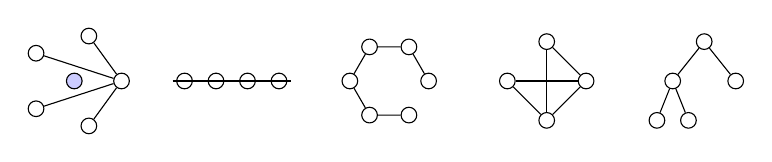
\begin{tikzpicture}[scale=0.5, every node/.style={circle,draw,inner sep=2pt}]
        % Star
        \node (s0) at (0,0) [fill=blue!20] {};
        \foreach \a in {0,72,...,288} \node (s\a) at (\a:1.2) {};
        \foreach \a in {0,72,...,288} \draw (s0)--(s\a);
        
        % Bus
        \begin{scope}[xshift=4cm]
            \draw[thick] (-1.5,0)--(1.5,0);
            \foreach \x in {-1.2,-0.4,0.4,1.2} \node at (\x,0) {};
        \end{scope}
        
        % Ring
        \begin{scope}[xshift=8cm]
            \foreach \a in {0,60,...,300} \node (r\a) at (\a:1) {};
            \draw (r0)--(r60)--(r120)--(r180)--(r240)--(r300)--cycle;
        \end{scope}
        
        % Mesh
        \begin{scope}[xshift=12cm]
            \node (m1) at (0,1) {}; \node (m2) at (1,0) {}; \node (m3) at (0,-1) {}; \node (m4) at (-1,0) {};
            \draw (m1)--(m2)--(m3)--(m4)--cycle; \draw (m1)--(m3) (m2)--(m4);
        \end{scope}
        
        % Tree
        \begin{scope}[xshift=16cm]
            \node (t1) at (0,1) {}; \node (t2) at (-0.8,0) {}; \node (t3) at (0.8,0) {};
            \node (t4) at (-1.2,-1) {}; \node (t5) at (-0.4,-1) {};
            \draw (t1)--(t2) (t1)--(t3) (t2)--(t4) (t2)--(t5);
        \end{scope}
    \end{tikzpicture}
\end{frame}

\section{三种交换方式}

\begin{frame}{电路交换 --- 资源独占}
    \begin{columns}[T]
        \column{0.5\textwidth}
        \textbf{三个阶段}：
        \begin{enumerate}
            \item \textbf{建立连接}：拨号申请
            \item \textbf{数据传输}：占用专用通路
            \item \textbf{释放连接}：拆除通路
        \end{enumerate}
        \column{0.5\textwidth}
        \textbf{优缺点}：
        \begin{itemize}
            \item[\color{green!70!black}$\checkmark$] 实时性极佳，无冲突
            \item[\color{red!70!black}$\times$] \textbf{资源利用率极低}
            \item[\color{red!70!black}$\times$] 建立连接时间长
        \end{itemize}
    \end{columns}
    \vspace{1em}
    \begin{exampleblock}{形象类比}
        \textbf{打电话}：你接通电话后就算不说话，这条线别人也用不了。
    \end{exampleblock}
\end{frame}

\begin{frame}{报文交换 --- 存储转发}
    \begin{itemize}
        \item \textbf{过程}：源节点将整个报文发送给相邻节点，相邻节点收到并\textbf{全部存储}后，再转发给下一个节点。
        \item \textbf{优点}：动态分配带宽，提高利用率。
        \item \textbf{缺点}：时延大，对中间节点存储空间要求高。
    \end{itemize}
    \vspace{1em}
    \begin{exampleblock}{形象类比}
        \textbf{寄信}：你写一封厚厚的信丢进邮箱，邮局收齐后整袋转运。
    \end{exampleblock}
\end{frame}

\begin{frame}{分组交换 --- 现代网络基础}
    \begin{itemize}
        \item \textbf{核心思想}：将大报文切割为若干小的\textbf{分组}（Packet）。
        \item \textbf{机制}：存储转发。但因为分组小，存储时间短，时延大大降低。
        \item \textbf{分类}：
        \begin{enumerate}
            \item \textbf{数据报}（Datagram）：无连接，分组独立选路（互联网主流）。
            \item \textbf{虚电路}（Virtual Circuit）：逻辑连接，分组走固定路径。
        \end{enumerate}
    \end{itemize}
    \vspace{0.5em}
    \begin{exampleblock}{形象类比}
        \textbf{发快递}：大件家具拆成几个小包裹，每个包裹都有面单，独立运输。
    \end{exampleblock}
\end{frame}

\begin{frame}{分组交换详解：数据报 vs 虚电路}
    \begin{table}
        \small
        \begin{tabular}{|l|c|c|}
            \hline
            \textbf{特性} & \textbf{数据报方式} & \textbf{虚电路方式} \\ \hline
            连接建立 & \textbf{不需要} & \textbf{需要} \\
            分组路径 & 独立选择（可能乱序） & 固定路径（按序到达） \\
            故障响应 & 自动绕行 & 虚电路断开需重连 \\
            适用场景 & 互联网、非实时应用 & ATM、对质量有要求的场景 \\
            \hline
        \end{tabular}
    \end{table}
    \vspace{0.5em}
    \begin{block}{重要结论}
        TCP协议虽然提供"面向连接"的服务，但它是工作在\textbf{运输层}的，其底层的\textbf{网络层}仍然使用的是无连接的\textbf{数据报}分组交换。
    \end{block}
\end{frame}

\begin{frame}{三种交换方式总结对比}
    \centering
    \begin{tikzpicture}[scale=0.8, >=stealth]
        % Draw time lines
        \draw[thick,->] (0,4) -- (0,0) node[below] {主机A};
        \draw[thick,->] (4,4) -- (4,0) node[below] {交换机};
        \draw[thick,->] (8,4) -- (8,0) node[below] {主机B};
        \node at (-1,2) {时间 $t$};
        
        % Simplified illustration for Grouping (just symbolic)
        \node at (4,4.5) {\textbf{存储转发示意 (分组交换)}};
        \draw[blue, thick] (0,3.5) -- (4,3.0);
        \draw[blue, thick] (0,3.3) -- (4,2.8);
        \draw[blue, thick] (4,3.0) -- (8,2.5);
        \draw[blue, thick] (4,2.8) -- (8,2.3);
    \end{tikzpicture}
    \vspace{0.5em}
    \begin{enumerate}
        \item \textbf{电路交换}：建立连接 $\rightarrow$ 传输 $\rightarrow$ 释放。适合海量持续数据。
        \item \textbf{报文交换}：整个报文存储转发。已基本被淘汰。
        \item \textbf{分组交换}：小块数据存储转发。灵活性最高，时延最低。
    \end{enumerate}
\end{frame}

\begin{frame}{[例题] 电路交换与分组交换的时延比较}
    \textbf{题目}：传送1MB数据，链路速率1Mbps。电路交换建立时间100ms。分组交换分组长1000B（含头20B），共经3段链路（2个路由器）。求总时延（忽略传播/处理时延）。\\
    \vspace{0.5em}
    \textbf{解析}：
    \begin{enumerate}
        \item \textbf{电路交换}：$T = 100\text{ms} + \frac{1\text{MB} \times 8}{1\text{Mbps}} = 100\text{ms} + 8.3886\text{s} \approx 8.49\text{s}$
        \item \textbf{分组交换}：
        \begin{itemize}
            \item 分组数 $k = \frac{1\text{MB}}{1000-20\text{B}} \approx 1049$
            \item 发送时延 $t_s = \frac{1000 \times 8}{10^6} = 8\text{ms}$
            \item 最后一个分组到达需经过路由器转发：$(1049-1) \times 8\text{ms} + 3 \times 8\text{ms} \approx 8.416\text{s}$
        \end{itemize}
    \end{enumerate}
    \textbf{结论}：对于突发数据，分组交换通常更高效。
\end{frame}

\begin{frame}{本节总结}
    \begin{enumerate}
        \item \textbf{核心定义}：互连、自治、资源共享
        \item \textbf{分类}：PAN, LAN(MAC), MAN, WAN(IP)
        \item \textbf{拓扑}：星型、总线、环型、网状、树型
        \item \textbf{交换方式}：
        \begin{itemize}
            \item 电路交换（专线，效率低）
            \item 报文交换（整报存储）
            \item \textbf{分组交换}（小块转发，主流）
        \end{itemize}
        \item \textbf{数据报 vs 虚电路}：无连接与面向逻辑连接
    \end{enumerate}
\end{frame}

\end{document}


\subsection{4-2 网络性能指标}
\documentclass[10pt, aspectratio=169]{beamer}
\usepackage{../beamer_theme_408}
\title{408考研零基础 --- 计算机网络}
\subtitle{4-2 网络性能指标}
\author{}
\date{}
\begin{document}
\begin{frame}{本节目标}
    \begin{enumerate}
        \item 掌握速率、带宽、吞吐量的概念
        \item 理解四种时延及其计算
        \item 掌握时延带宽积和RTT的含义
        \item 理解信道利用率与时延的关系
    \end{enumerate}
\end{frame}

\begin{frame}{速率与带宽}
    \begin{columns}[T]
        \column{0.5\textwidth}
        \textbf{速率（Rate）}
        \begin{itemize}
            \item 指\textbf{实际}数据传送速率
            \item 单位：bps（bit/s）、kb/s、Mb/s、Gb/s
            \item 注意：$1$ kb/s = $10^3$ b/s
            \item 存储器中 $1$ KB = $2^{10}$ B
            \item 通信中 $1$ kb/s = $10^3$ b/s
            \item 考研中\textbf{特别注意}换算！
        \end{itemize}
        \column{0.5\textwidth}
        \textbf{带宽（Bandwidth）}
        \begin{itemize}
            \item 原意：信号频率范围（Hz）
            \item 计网中指\textbf{最高}数据速率
            \item 单位：bps
            \item 表示网络通信\textbf{能力}的上限
        \end{itemize}
    \end{columns}
    \vspace{0.5em}
    \begin{exampleblock}{对比}
        带宽就像公路的\textbf{限速}，速率就像汽车当前的\textbf{实际速度}。
    \end{exampleblock}
\end{frame}

\begin{frame}{吞吐量}
    \begin{itemize}
        \item \textbf{定义}：单位时间内通过某个网络（或信道、接口）的\textbf{实际}数据量
        \item 单位：bps
        \item 受网络带宽和当前网络负载的\textbf{限制}
    \end{itemize}
    \vspace{0.5em}
    \begin{exampleblock}{理解}
        \begin{itemize}
            \item 带宽 = \textbf{理论最高}可达速率
            \item 吞吐量 = \textbf{实际}达到的速率
            \item 吞吐量 $\le$ 带宽
            \item 例：100Mbps的以太网，实际吞吐量可能只有40Mbps
        \end{itemize}
    \end{exampleblock}
    \vspace{0.3em}
    \begin{block}{考研提示}
        区分"带宽"（理论最大值）和"吞吐量"（实际测量值）。
    \end{block}
\end{frame}

\begin{frame}{时延 --- 概述}
    \textbf{时延（Delay / Latency）}：数据从网络一端传输到另一端所需的总时间。\\
    \vspace{0.3em}
    由四部分组成：
    \begin{enumerate}
        \item \textbf{发送时延}（传输时延）
        \item \textbf{传播时延}
        \item \textbf{处理时延}
        \item \textbf{排队时延}
    \end{enumerate}
    \vspace{0.5em}
    \begin{block}{总时延公式}
        \begin{center}
            \Large
            $\text{总时延} = \text{发送时延} + \text{传播时延} + \text{处理时延} + \text{排队时延}$
        \end{center}
    \end{block}
\end{frame}

\begin{frame}{发送时延与传播时延}
    \begin{columns}[T]
        \column{0.5\textwidth}
        \textbf{发送时延}
        \begin{itemize}
            \item 从发送第一个bit到最后一个bit发出所需时间
            \item 公式：
            $$\text{发送时延} = \frac{\text{数据长度}}{\text{带宽}}$$
            \item 取决于\textbf{数据长度}和\textbf{发送速率}
        \end{itemize}
        \vspace{0.5em}
        \textbf{何时为主要因素？}
        \begin{itemize}
            \item 数据量大时，发送时延占主导
        \end{itemize}
        \column{0.5\textwidth}
        \textbf{传播时延}
        \begin{itemize}
            \item 数据在信道上传播所需时间
            \item 公式：
            $$\text{传播时延} = \frac{\text{信道长度}}{\text{传播速度}}$$
            \item 取决于\textbf{物理介质}和\textbf{距离}
        \end{itemize}
        \vspace{0.5em}
        \textbf{何时为主要因素？}
        \begin{itemize}
            \item 长距离时，传播时延占主导
        \end{itemize}
    \end{columns}
    \vspace{0.3em}
    \begin{block}{传播速度}
        光速 $3\times10^8$m/s（真空中），在铜缆中约 $2.3\times10^8$m/s，在光纤中约 $2.0\times10^8$m/s。
    \end{block}
\end{frame}

\begin{frame}{处理时延与排队时延}
    \begin{columns}[T]
        \column{0.5\textwidth}
        \textbf{处理时延}
        \begin{itemize}
            \item 路由器/交换机检查分组首部、查路由表等处理的时间
            \item 通常很小，但在高负载下可能增加
            \item 与设备性能相关
        \end{itemize}
        \column{0.5\textwidth}
        \textbf{排队时延}
        \begin{itemize}
            \item 分组在路由器输入/输出队列中等待的时间
            \item 取决于网络拥塞程度
            \item 变化最大，最不可预测
            \item 当网络负载接近容量时急剧增加
        \end{itemize}
    \end{columns}
    \vspace{0.5em}
    \begin{exampleblock}{记忆口诀}
        "发送靠长度，传播靠距离，处理看设备，排队看拥塞"
    \end{exampleblock}
\end{frame}

\begin{frame}{时延带宽积}
    \begin{block}{定义}
        \textbf{时延带宽积} = \textbf{传播时延} $\times$ \textbf{带宽}
    \end{block}
    \vspace{0.3em}
    \begin{itemize}
        \item 含义：以\textbf{比特}为单位的链路长度
        \item 表示\textbf{信道中最多能容纳的比特数}
        \item 类似于管道的\textbf{容积}
    \end{itemize}
    \vspace{0.5em}
    \begin{exampleblock}{类比理解}
        水管长度 = 传播时延，水管粗细 = 带宽，时延带宽积 = 水管中的水量
    \end{exampleblock}
    \vspace{0.3em}
    \begin{block}{考研常考}
        若时延带宽积为 $L$ bit，则发送方在收到第一个比特确认前最多能发送 $L$ bit。
    \end{block}
\end{frame}

\begin{frame}{RTT（往返时间）}
    \begin{block}{定义}
        \textbf{RTT（Round-Trip Time）}：数据从发送端发送开始，到收到来自接收端的确认所经历的时间。
    \end{block}
    \vspace{0.5em}
    \begin{itemize}
        \item 包括：传播时延 $\times$ 2 + 处理时延（收发双方）+ 排队时延
        \item 注意：RTT \textbf{不包含}发送时延
    \end{itemize}
    \vspace{0.5em}
    \begin{exampleblock}{举例}
        发送方发送一个分组到接收方，接收方立即回复确认，发送方收到确认的总时间就是RTT。
    \end{exampleblock}
    \vspace{0.3em}
    \begin{block}{有效数据率}
        $$\text{有效数据率} = \frac{\text{数据长度}}{\text{发送时延} + \text{RTT}}$$
    \end{block}
\end{frame}

\begin{frame}{信道利用率与网络利用率}
    \begin{columns}[T]
        \column{0.5\textwidth}
        \textbf{信道利用率}
        \begin{itemize}
            \item 数据通过时间 / 总时间
            \item 公式：
            $$\text{信道利用率} = \frac{\text{数据通过时间}}{T_{\text{总}}}$$
            \item 反映信道被有效利用的程度
        \end{itemize}
        \column{0.5\textwidth}
        \textbf{网络利用率}
        \begin{itemize}
            \item 各信道利用率的\textbf{加权平均值}
            \item 反映整个网络的负载情况
            \item 利用率越高，网络负载越重
        \end{itemize}
    \end{columns}
    \vspace{0.5em}
    \begin{alertblock}{注意}
        利用率并非越高越好！利用率过高会导致时延急剧增大。
    \end{alertblock}
\end{frame}

\begin{frame}{时延与利用率的关系}
    \begin{block}{关键公式}
        \begin{center}
            \Large
            $D = \dfrac{D_0}{1 - U}$
        \end{center}
    \end{block}
    \vspace{0.3em}
    \begin{itemize}
        \item $D$：当前网络时延
        \item $D_0$：空闲时的时延（$U=0$）
        \item $U$：网络利用率（$0 \le U < 1$）
    \end{itemize}
    \vspace{0.5em}
    \begin{exampleblock}{规律}
        \begin{itemize}
            \item 当 $U=0$ 时，$D=D_0$（最小时延）
            \item 当 $U\to 1$ 时，$D\to \infty$（时延急剧增大）
            \item 利用率越高，时延越大！
        \end{itemize}
    \end{exampleblock}
    \vspace{0.3em}
    \begin{block}{考研提示}
        不能片面追求高利用率，需要在利用率和时延之间做出权衡。
    \end{block}
\end{frame}

\begin{frame}{本节总结}
    \begin{enumerate}
        \item \textbf{速率}（实际速率）与\textbf{带宽}（最高速率）
        \item \textbf{吞吐量}：实际测量值 $\le$ 带宽
        \item \textbf{时延}：发送时延 + 传播时延 + 处理时延 + 排队时延
        \item \textbf{发送时延} = 数据长/带宽，\textbf{传播时延} = 距离/传播速度
        \item \textbf{时延带宽积} = 传播时延 $\times$ 带宽（比特计数的链路长度）
        \item \textbf{RTT}：数据发送到收到确认的时间（不含发送时延）
        \item 利用率 $U$ 越高，时延 $D = D_0/(1-U)$ 越大
    \end{enumerate}
\end{frame}
\end{document}


\subsection{4-3 网络体系结构}
\documentclass[10pt, aspectratio=169]{beamer}
\usepackage{../beamer_theme_408}
\title{408考研零基础 --- 计算机网络}
\subtitle{4-3 网络体系结构}
\author{}
\date{}
\begin{document}
\begin{frame}{本节目标}
    \begin{enumerate}
        \item 理解分层思想和分层的优点
        \item 掌握OSI七层模型及各层功能
        \item 掌握TCP/IP四层模型
        \item 理解五层参考模型及各层PDU
        \item 理解封装与解封装过程
    \end{enumerate}
\end{frame}

\begin{frame}{分层思想}
    \begin{block}{为什么需要分层？}
        计算机网络是一个复杂的系统，分层可以将复杂问题分解为若干个较小的、易于处理的子问题。
    \end{block}
    \vspace{0.3em}
    \textbf{分层的优点}：
    \begin{enumerate}
        \item \textbf{各层独立}：每层完成特定功能，修改某一层不影响其他层
        \item \textbf{接口清晰}：相邻层之间有明确的交互接口
        \item \textbf{灵活性好}：某一层变化不影响其他层，便于技术更新
        \item \textbf{易于实现和维护}：将复杂系统分解为简单模块
    \end{enumerate}
    \vspace{0.3em}
    \begin{exampleblock}{类比}
        类似于邮政系统：写信（应用层）$\rightarrow$ 装信封（表示层）$\rightarrow$ 投递（传输层）$\rightarrow$ 分拣（网络层）
    \end{exampleblock}
\end{frame}

\begin{frame}{OSI七层模型}
    \begin{columns}[T]
        \column{0.6\textwidth}
        \textbf{OSI七层（从下到上）}：
        \begin{enumerate}
            \item \textbf{物理层}：传输比特流，定义接口特性
            \item \textbf{数据链路层}：封装成帧，差错控制，流量控制
            \item \textbf{网络层}：路由选择，分组转发，拥塞控制
            \item \textbf{传输层}：端到端通信，可靠传输
            \item \textbf{会话层}：会话管理，同步
            \item \textbf{表示层}：数据格式转换，加密压缩
            \item \textbf{应用层}：用户接口，网络服务
        \end{enumerate}
        \column{0.4\textwidth}
        \begin{block}{记忆口诀}
            "物链网传会表应"\\
            \vspace{0.3em}
            \small
            物理层 $\to$ 链路层 $\to$ 网络层 $\to$ 传输层 $\to$ 会话层 $\to$ 表示层 $\to$ 应用层
        \end{block}
        \vspace{0.5em}
        \begin{alertblock}{注意}
            OSI是法律上的国际标准，但并未在实际中完全采用。
        \end{alertblock}
    \end{columns}
\end{frame}

\begin{frame}{OSI模型各层功能详解}
    \begin{table}
        \begin{tabular}{|c|l|}
            \hline
            \textbf{层次} & \textbf{主要功能} \\ \hline
            应用层 & 提供用户接口，如HTTP、FTP、SMTP、DNS \\
            表示层 & 数据格式转换、加密/解密、压缩/解压缩 \\
            会话层 & 建立/管理/终止会话，同步点 \\
            传输层 & 端到端通信，可靠传输（TCP）/不可靠（UDP） \\
            网络层 & 路由选择、分组转发、逻辑寻址（IP地址） \\
            数据链路层 & 封装成帧、差错检测（CRC）、流量控制 \\
            物理层 & 定义机械/电气/功能/规程特性，传输比特流 \\
            \hline
        \end{tabular}
    \end{table}
    \vspace{0.3em}
    \begin{block}{考研常考}
        各层的功能区分和典型协议是选择题高频考点。
    \end{block}
\end{frame}

\begin{frame}{TCP/IP四层模型}
    \begin{columns}[T]
        \column{0.5\textwidth}
        \textbf{TCP/IP四层（从下到上）}：
        \begin{enumerate}
            \item \textbf{网络接口层}
            \begin{itemize}
                \item 对应OSI的物理层+数据链路层
                \item 无明确规定，与具体物理网络相关
            \end{itemize}
            \item \textbf{网际层}
            \begin{itemize}
                \item 对应OSI的网络层
                \item 核心协议：\textbf{IP协议}
            \end{itemize}
            \item \textbf{传输层}
            \begin{itemize}
                \item 对应OSI的传输层
                \item 核心协议：\textbf{TCP、UDP}
            \end{itemize}
            \item \textbf{应用层}
            \begin{itemize}
                \item 对应OSI的会话层+表示层+应用层
                \item 包含所有高层协议
            \end{itemize}
        \end{enumerate}
        \column{0.5\textwidth}
        \begin{block}{特点}
            \begin{itemize}
                \item TCP/IP是\textbf{事实上的国际标准}
                \item Internet的基础协议
                \item 比OSI更简洁实用
                \item 网际层（IP层）是核心
            \end{itemize}
        \end{block}
    \end{columns}
\end{frame}

\begin{frame}{五层参考模型（综合）}
    \begin{columns}[T]
        \column{0.55\textwidth}
        结合OSI和TCP/IP优点的\textbf{五层模型}：
        \begin{enumerate}
            \item \textbf{物理层}：传输比特流
            \item \textbf{数据链路层}：封装成帧
            \item \textbf{网络层}：路由转发
            \item \textbf{传输层}：端到端通信
            \item \textbf{应用层}：用户服务
        \end{enumerate}
        \vspace{0.5em}
        \textcolor{blue}{\textbf{408考研采用五层参考模型！}}
        \column{0.45\textwidth}
        \begin{table}
            \small
            \begin{tabular}{|c|c|}
                \hline
                \textbf{五层模型} & \textbf{对应OSI} \\ \hline
                应用层 & 应用+表示+会话 \\
                传输层 & 传输层 \\
                网络层 & 网络层 \\
                数据链路层 & 数据链路层 \\
                物理层 & 物理层 \\
                \hline
            \end{tabular}
        \end{table}
    \end{columns}
\end{frame}

\begin{frame}{PDU（协议数据单元）}
    \begin{block}{定义}
        \textbf{PDU（Protocol Data Unit）}：不同层次的数据单位，每层对数据有特定的称呼。
    \end{block}
    \vspace{0.5em}
    \begin{table}
        \begin{tabular}{|c|c|c|}
            \hline
            \textbf{层次} & \textbf{PDU名称} & \textbf{备注} \\ \hline
            应用层 & \textbf{报文（Message）} & HTTP、FTP等协议的数据 \\
            传输层 & \textbf{报文段（Segment）} & TCP段 / UDP数据报 \\
            网络层 & \textbf{数据报/包（Packet）} & IP数据报 \\
            数据链路层 & \textbf{帧（Frame）} & 包含MAC地址 \\
            物理层 & \textbf{比特流（Bitstream）} & 原始的0/1信号 \\
            \hline
        \end{tabular}
    \end{table}
    \vspace{0.3em}
    \begin{block}{考研常考}
        请牢记各层PDU名称，这是408高频考点！
    \end{block}
\end{frame}

\begin{frame}{封装与解封装}
    \begin{columns}[T]
        \column{0.5\textwidth}
        \textbf{封装（发送方）}：
        \begin{itemize}
            \item 应用层：产生报文（Message）
            \item 传输层：加TCP/UDP头部 $\to$ 报文段
            \item 网络层：加IP头部 $\to$ 数据报
            \item 数据链路层：加MAC头部+尾部 $\to$ 帧
            \item 物理层：转为比特流发送
        \end{itemize}
        \column{0.5\textwidth}
        \textbf{解封装（接收方）}：
        \begin{itemize}
            \item 物理层：接收比特流
            \item 数据链路层：去掉帧头和帧尾 $\to$ 数据报
            \item 网络层：去掉IP头部 $\to$ 报文段
            \item 传输层：去掉TCP/UDP头部 $\to$ 报文
            \item 应用层：读取数据
        \end{itemize}
    \end{columns}
    \vspace{0.5em}
    \begin{exampleblock}{关键理解}
        每层只处理本层的头部信息，下层对上层是透明的！
    \end{exampleblock}
\end{frame}

\begin{frame}{三个模型的层次对应关系}
    \begin{table}
        \begin{tabular}{|c|c|c|c|}
            \hline
            \textbf{层次} & \textbf{OSI七层} & \textbf{TCP/IP四层} & \textbf{五层参考模型} \\ \hline
            7 & 应用层 & \multirow{3}{*}{应用层} & \multirow{3}{*}{应用层} \\
            6 & 表示层 & & \\
            5 & 会话层 & & \\
            4 & 传输层 & 传输层 & 传输层 \\
            3 & 网络层 & 网际层 & 网络层 \\
            2 & 数据链路层 & \multirow{2}{*}{网络接口层} & 数据链路层 \\
            1 & 物理层 & & 物理层 \\
            \hline
        \end{tabular}
    \end{table}
    \vspace{0.5em}
    \begin{center}
        \textcolor{blue}{408考研复习以\textbf{五层参考模型}为主线}
    \end{center}
\end{frame}

\begin{frame}{本节总结}
    \begin{enumerate}
        \item \textbf{分层思想}：各层独立、接口清晰、灵活性好
        \item \textbf{OSI七层}：物、链、网、传、会、表、应
        \item \textbf{TCP/IP四层}：网络接口、网际、传输、应用
        \item \textbf{五层参考模型}（408采用）：物理、链路、网络、传输、应用
        \item \textbf{PDU}：报文 $\to$ 报文段 $\to$ 数据报 $\to$ 帧 $\to$ 比特流
        \item 发送方\textbf{封装}（加头），接收方\textbf{解封装}（去头）
    \end{enumerate}
\end{frame}
\end{document}


\subsection{4-4 物理层基础}
\documentclass[10pt, aspectratio=169]{beamer}
\usepackage{../beamer_theme_408}
\title{408考研零基础 --- 计算机网络}
\subtitle{4-4 物理层基础}
\author{}
\date{}
\begin{document}
\frame{\titlepage}
\begin{frame}{本节目标}
    \begin{enumerate}
        \item 理解物理层的任务和四大特性
        \item 掌握信源、信道、信宿和信号分类
        \item 理解码元、码元速率（波特率）的概念
        \item 掌握奈奎斯特定理和香农定理
        \item 掌握信噪比的计算
    \end{enumerate}
\end{frame}

\begin{frame}{物理层的任务}
    \begin{block}{物理层的作用}
        在连接各计算机的传输媒体上传输\textbf{比特流}（0和1），为数据链路层提供透明的比特流传输服务。
    \end{block}
    \vspace{0.5em}
    \textbf{物理层的四大特性}：
    \begin{enumerate}
        \item \textbf{机械特性}：接口的形状、尺寸、引脚数等物理规格
        \item \textbf{电气特性}：电压高低、电流大小等电气参数
        \item \textbf{功能特性}：各条信号线的用途（数据线、控制线等）
        \item \textbf{规程特性}：信号线上事件的顺序（时序）
    \end{enumerate}
    \vspace{0.3em}
    \begin{exampleblock}{举例}
        RJ45接口（网口）的物理尺寸属于机械特性，引脚电压范围属于电气特性。
    \end{exampleblock}
\end{frame}

\begin{frame}{通信基本概念}
    \begin{columns}[T]
        \column{0.5\textwidth}
        \textbf{三个基本要素}：
        \begin{itemize}
            \item \textbf{信源}：产生和发送数据的源设备
            \item \textbf{信道}：信号传输的介质通路
            \item \textbf{信宿}：接收数据的目的设备
        \end{itemize}
        \vspace{0.5em}
        \begin{center}
            \begin{tikzpicture}[scale=0.5]
                \node[draw,rectangle,minimum width=1.5cm,minimum height=0.8cm] (s) at (-3,0) {信源};
                \node[draw,rectangle,minimum width=1.5cm,minimum height=0.8cm] (c) at (0,0) {信道};
                \node[draw,rectangle,minimum width=1.5cm,minimum height=0.8cm] (d) at (3,0) {信宿};
                \draw[->,thick] (s)--(c);
                \draw[->,thick] (c)--(d);
            \end{tikzpicture}
        \end{center}
        \column{0.5\textwidth}
        \textbf{信号分类}：
        \begin{itemize}
            \item \textbf{模拟信号}：连续变化的信号（如声音）
            \item \textbf{数字信号}：离散的信号（0/1）
        \end{itemize}
        \vspace{0.5em}
        \begin{block}{信道分类}
            \begin{itemize}
                \item 单向信道（单工）
                \item 双向交替信道（半双工）
                \item 双向同时信道（全双工）
            \end{itemize}
        \end{block}
    \end{columns}
\end{frame}

\begin{frame}{码元与波特率}
    \begin{block}{码元（Symbol / Code Element）}
        信号的基本波形单位。一个码元可以携带多个比特的信息。
    \end{block}
    \vspace{0.3em}
    \begin{columns}[T]
        \column{0.5\textwidth}
        \textbf{相关概念}：
        \begin{itemize}
            \item \textbf{码元速率}（波特率，$Baud$）：每秒传输的码元个数，单位\textbf{Baud}
            \item \textbf{数据速率}（比特率，$R$）：每秒传输的比特数，单位\textbf{bps}
        \end{itemize}
        \column{0.5\textwidth}
        \textbf{两者关系}：
        $$R = B \cdot \log_2 V$$
        \begin{itemize}
            \item $B$：波特率（Baud）
            \item $V$：每个码元的状态数
            \item $R$：数据率（bps）
        \end{itemize}
    \end{columns}
    \vspace{0.5em}
    \begin{exampleblock}{举例}
        若 $V=4$（每个码元代表4种状态=2bit），$B=1000$Baud，则 $R = 1000 \times \log_2 4 = 2000$bps。
    \end{exampleblock}
\end{frame}

\begin{frame}{奈奎斯特定理（无噪声）}
    \begin{block}{定理内容}
        在\textbf{无噪声}的理想信道中，\textbf{极限码元速率}为 $2W$（Baud），其中 $W$ 是信道的带宽（Hz）。
    \end{block}
    \vspace{0.3em}
    \textbf{公式}：
    \begin{itemize}
        \item \textbf{极限码元速率} $= 2W$（Baud）
        \item \textbf{极限数据速率} $= 2W \log_2 V$（bps）
    \end{itemize}
    \vspace{0.5em}
    \begin{exampleblock}{例题}
        某信道带宽为 4kHz，使用 16 种状态码元，求极限数据率？\\
        \textbf{解}：$R_{\max} = 2 \times 4000 \times \log_2 16 = 8000 \times 4 = 32$kbps
    \end{exampleblock}
    \vspace{0.3em}
    \begin{alertblock}{注意}
        奈奎斯特定理只考虑\textbf{无噪声}的理想情况，给出了上限。
    \end{alertblock}
\end{frame}

\begin{frame}{香农定理（有噪声）}
    \begin{block}{定理内容}
        在\textbf{有噪声}的实际信道中，极限数据速率受信噪比限制。
    \end{block}
    \vspace{0.3em}
    \textbf{公式}：
    $$C = W \cdot \log_2(1 + S/N)$$
    \begin{itemize}
        \item $C$：极限数据速率（bps）
        \item $W$：信道带宽（Hz）
        \item $S/N$：\textbf{信噪比}（信号功率/噪声功率，无量纲）
    \end{itemize}
    \vspace{0.5em}
    \begin{block}{信噪比（dB）换算}
        $$\text{信噪比(dB)} = 10\log_{10}(S/N)$$
        \vspace{-0.5em}
        $$S/N = 10^{\frac{\text{信噪比(dB)}}{10}}$$
    \end{block}
\end{frame}

\begin{frame}{信噪比计算示例}
    \begin{exampleblock}{例题1}
        已知信噪比为 30dB，带宽为 3kHz，求最大数据率？\\
        \textbf{解}：
        \begin{align*}
            30\text{dB} &= 10\log_{10}(S/N) \\
            \log_{10}(S/N) &= 3 \\
            S/N &= 10^3 = 1000 \\
            C &= 3000 \times \log_2(1 + 1000) \\
            &\approx 3000 \times \log_2 1001 \approx 3000 \times 9.97 \approx 29.9\text{kbps}
        \end{align*}
    \end{exampleblock}
    \vspace{0.3em}
    \begin{exampleblock}{例题2}
        某信道带宽 4kHz，信噪比 40dB，求极限数据率？\\
        \textbf{解}：$S/N = 10^{40/10} = 10^4 = 10000$，$C = 4000 \times \log_2(10001) \approx 53.1$kbps
    \end{exampleblock}
\end{frame}

\begin{frame}{奈奎斯特 vs 香农}
    \begin{table}
        \begin{tabular}{|c|c|c|}
            \hline
            \textbf{对比项} & \textbf{奈奎斯特定理} & \textbf{香农定理} \\ \hline
            适用条件 & 无噪声理想信道 & 有噪声实际信道 \\
            考虑因素 & 带宽 $W$、码元状态 $V$ & 带宽 $W$、信噪比 $S/N$ \\
            公式 & $2W\log_2 V$ & $W\log_2(1+S/N)$ \\
            意义 & 限制码元速率 & 限制数据速率 \\
            应用 & 确定码元状态数 & 确定极限传输速率 \\
            \hline
        \end{tabular}
    \end{table}
    \vspace{0.5em}
    \begin{block}{考研常考思路}
        \begin{enumerate}
            \item 先由香农定理求出极限速率 $C$
            \item 再由奈奎斯特定理 $C = 2W\log_2 V$ 反推 $V$
        \end{enumerate}
    \end{block}
\end{frame}

\begin{frame}{本节总结}
    \begin{enumerate}
        \item 物理层任务：传输比特流，定义\textbf{机械、电气、功能、规程}四大特性
        \item 通信三要素：\textbf{信源、信道、信宿}
        \item 码元速率（Baud）与数据率（bps）关系：$R = B \cdot \log_2 V$
        \item \textbf{奈奎斯特定理}（无噪）：$R_{\max} = 2W\log_2 V$
        \item \textbf{香农定理}（有噪）：$C = W\log_2(1+S/N)$
        \item 信噪比换算：$\text{dB} = 10\log_{10}(S/N)$
    \end{enumerate}
    \vspace{1em}
    \begin{center}
        \textcolor{blue}{\textbf{下节预告：4-5 传输介质与设备}}
    \end{center}
\end{frame}
\end{document}


\subsection{4-5 传输介质与设备}
\documentclass[10pt, aspectratio=169]{beamer}
\usepackage{../beamer_theme_408}
\title{408考研零基础 --- 计算机网络}
\subtitle{4-5 传输介质与设备}
\author{}
\date{}
\begin{document}
\begin{frame}{本节目标}
    \begin{enumerate}
        \item 掌握导向型传输介质的特点和应用
        \item 了解非导向型传输介质
        \item 掌握中继器和集线器的工作原理
        \item 理解冲突域的概念
    \end{enumerate}
\end{frame}

\begin{frame}{导向型传输介质 --- 双绞线}
    \begin{columns}[T]
        \column{0.55\textwidth}
        \textbf{双绞线}
        \begin{itemize}
            \item 将两根相互绝缘的铜导线\textbf{绞合}在一起
            \item 绞合目的：减少电磁干扰
            \item 接口：\textbf{RJ45}（水晶头）
        \end{itemize}
        \vspace{0.3em}
        \textbf{分类}：
        \begin{itemize}
            \item \textbf{STP}（屏蔽双绞线）：有金属屏蔽层，抗干扰强，成本高
            \item \textbf{UTP}（非屏蔽双绞线）：无屏蔽层，成本低，使用广泛
        \end{itemize}
        \vspace{0.3em}
        \textbf{常见标准}：Cat5e、Cat6（百兆/千兆以太网）
        \column{0.45\textwidth}
        \begin{block}{特点}
            \begin{itemize}
                \item[\color{green!70!black}$\checkmark$] 价格便宜，易于安装
                \item[\color{green!70!black}$\checkmark$] 适合短距离（$\le 100$m）
                \item[\color{red!70!black}$\times$] 传输距离有限
                \item[\color{red!70!black}$\times$] 易受电磁干扰
            \end{itemize}
        \end{block}
    \end{columns}
\end{frame}

\begin{frame}{导向型传输介质 --- 同轴电缆}
    \begin{columns}[T]
        \column{0.55\textwidth}
        \textbf{同轴电缆}
        \begin{itemize}
            \item 由内导体、绝缘层、外导体（屏蔽层）、外护套组成
            \item 外导体接地，抗干扰能力强
            \item 比双绞线传输距离更远
        \end{itemize}
        \vspace{0.3em}
        \textbf{分类}：
        \begin{itemize}
            \item \textbf{基带同轴电缆}（50$\Omega$）：传输数字信号，LAN中使用
            \item \textbf{宽带同轴电缆}（75$\Omega$）：传输模拟信号，有线电视
        \end{itemize}
        \column{0.45\textwidth}
        \begin{block}{特点}
            \begin{itemize}
                \item[\color{green!70!black}$\checkmark$] 抗干扰能力强
                \item[\color{green!70!black}$\checkmark$] 传输距离较远
                \item[\color{red!70!black}$\times$] 成本较高
                \item[\color{red!70!black}$\times$] 安装较复杂
            \end{itemize}
        \end{block}
    \end{columns}
\end{frame}

\begin{frame}{导向型传输介质 --- 光纤}
    \textbf{原理}：利用光的\textbf{全反射}特性，在玻璃纤维中传输光信号。
    \vspace{0.5em}
    \begin{columns}[T]
        \column{0.5\textwidth}
        \textbf{单模光纤}
        \begin{itemize}
            \item 纤芯很细（$8\sim10\mu$m）
            \item 光沿直线传播
            \item 衰减小，传输距离长（$>10$km）
            \item 成本高
            \item 适合远距离骨干网
        \end{itemize}
        \column{0.5\textwidth}
        \textbf{多模光纤}
        \begin{itemize}
            \item 纤芯较粗（$50\sim62.5\mu$m）
            \item 光以多个角度反射传播
            \item 有模间色散
            \item 距离较短（$<2$km）
            \item 成本低
            \item 适合局域网
        \end{itemize}
    \end{columns}
    \vspace{0.3em}
    \begin{block}{光纤优点}
        传输带宽高、损耗小、抗电磁干扰、保密性好
    \end{block}
\end{frame}

\begin{frame}{非导向型传输介质}
    \begin{columns}[T]
        \column{0.33\textwidth}
        \textbf{无线电波}
        \begin{itemize}
            \item 穿透性好
            \item 全方向传播
            \item 传输距离远
            \item WiFi、蓝牙、手机信号
            \item 易受干扰
        \end{itemize}
        \column{0.33\textwidth}
        \textbf{微波}
        \begin{itemize}
            \item 直线传播（视距）
            \item 频率高，带宽大
            \item 需中继站接力
            \item 对障碍物敏感
            \item 卫星通信、地面微波
        \end{itemize}
        \column{0.33\textwidth}
        \textbf{红外}
        \begin{itemize}
            \item 短距离通信
            \item 不能穿透障碍物
            \item 点对点
            \item 遥控器
            \item 成本低
        \end{itemize}
    \end{columns}
    \vspace{0.5em}
    \begin{block}{对比}
        无线电波穿透性好但速率较低，微波速率高但需要视距传输，红外适合短距离低成本场景。
    \end{block}
\end{frame}

\begin{frame}{物理层设备 --- 中继器}
    \begin{columns}[T]
        \column{0.55\textwidth}
        \textbf{中继器（Repeater）}
        \begin{itemize}
            \item 功能：对信号进行\textbf{再生和放大}，延长传输距离
            \item 工作在\textbf{物理层}
            \item 两端连接相同的网段
            \item 不能连接不同速率/协议的网段
        \end{itemize}
        \vspace{0.3em}
        \textbf{5-4-3规则}：
        \begin{itemize}
            \item 最多\textbf{5}个网段
            \item 最多\textbf{4}个中继器
            \item 最多\textbf{3}个网段有主机
        \end{itemize}
        \column{0.45\textwidth}
        \begin{block}{注意}
            \begin{itemize}
                \item 中继器不能连接不同类型的网络
                \item 不能过滤数据
                \item 将信号原样转发（包括噪声）
                \item 扩展了冲突域
            \end{itemize}
        \end{block}
    \end{columns}
\end{frame}

\begin{frame}{物理层设备 --- 集线器}
    \begin{columns}[T]
        \column{0.55\textwidth}
        \textbf{集线器（Hub）}
        \begin{itemize}
            \item 本质：\textbf{多端口的中继器}
            \item 工作在\textbf{物理层}
            \item 接收一个端口信号，向\textbf{所有其他端口}转发
            \item \textbf{共享带宽}：所有端口平分总带宽
            \item \textbf{半双工}：同一时刻只能单向传输
        \end{itemize}
        \vspace{0.3em}
        \begin{alertblock}{重要特性}
            集线器连接的设备处于同一个\textbf{冲突域}和\textbf{广播域}。
        \end{alertblock}
        \column{0.45\textwidth}
        \begin{exampleblock}{举例}
            10Mbps的集线器连接4台主机：\\
            $\to$ 总带宽10Mbps共享\\
            $\to$ 每台主机理论最高10Mbps\\
            $\to$ 但实际需竞争，总带宽固定10Mbps
        \end{exampleblock}
    \end{columns}
\end{frame}

\begin{frame}{冲突域的概念}
    \begin{block}{冲突域（Collision Domain）}
        当两$+$台设备同时发送数据时，信号会在共享介质上产生\textbf{冲突}的范围。
    \end{block}
    \vspace{0.3em}
    \begin{columns}[T]
        \column{0.5\textwidth}
        \textbf{冲突域的特点}：
        \begin{itemize}
            \item 共享同一传输介质的所有设备
            \item 同一时刻只能一台设备发送
            \item 冲突发生时需重传
            \item 降低网络效率
        \end{itemize}
        \column{0.5\textwidth}
        \textbf{设备对冲突域的影响}：
        \begin{itemize}
            \item \textbf{集线器/中继器}：不隔离冲突域
            \item \textbf{交换机/网桥}：隔离冲突域（每个端口独立冲突域）
            \item \textbf{路由器}：隔离冲突域和广播域
        \end{itemize}
    \end{columns}
    \vspace{0.5em}
    \begin{exampleblock}{区分}
        \textbf{冲突域}：物理层概念，共享介质产生冲突的范围\\
        \textbf{广播域}：网络层概念，能收到广播的范围
    \end{exampleblock}
\end{frame}

\begin{frame}{本节总结}
    \begin{enumerate}
        \item \textbf{导向型介质}：双绞线（STP/UTP，RJ45）、同轴电缆（基带/宽带）、光纤（单模/多模，全反射）
        \item \textbf{非导向型介质}：无线电波（穿透好）、微波（直线中继）、红外（短距离）
        \item \textbf{中继器}：信号再生放大，延长距离；5-4-3规则
        \item \textbf{集线器}：多端口中继器，共享带宽，半双工
        \item \textbf{冲突域}：共享介质时信号冲突的范围；集线器不隔离冲突域
    \end{enumerate}
\end{frame}
\end{document}


\subsection{4-6 数据链路层功能}
\documentclass[10pt, aspectratio=169]{beamer}
\usepackage{../beamer_theme_408}
\title{408考研零基础 --- 计算机网络}
\subtitle{4-6 数据链路层功能}
\author{}
\date{}
\begin{document}
\frame{\titlepage}
\begin{frame}{本节目标}
    \begin{enumerate}
        \item 掌握数据链路层的五大功能
        \item 理解封装成帧和透明传输
        \item 掌握CRC循环冗余校验原理
        \item 区分检错与纠错
        \item 理解滑动窗口机制的基本概念
    \end{enumerate}
\end{frame}

\begin{frame}{数据链路层功能概述}
    \begin{block}{定位}
        数据链路层位于\textbf{物理层之上、网络层之下}，负责在相邻节点间的链路上可靠地传输数据。
    \end{block}
    \vspace{0.3em}
    \textbf{五大功能}：
    \begin{enumerate}
        \item \textbf{封装成帧}：将网络层的数据报加上首部和尾部，形成帧
        \item \textbf{透明传输}：确保数据中任何比特组合都能正常传输
        \item \textbf{差错控制}：检测和纠正传输过程中的比特错误
        \item \textbf{流量控制}：协调发送方和接收方的速率
        \item \textbf{链路管理}：建立、维护和释放数据链路
    \end{enumerate}
    \vspace{0.3em}
    \begin{exampleblock}{类比}
        数据链路层相当于快递的\textbf{分拣和运输环节}，负责将包裹（帧）从一个站点送到相邻站点。
    \end{exampleblock}
\end{frame}

\begin{frame}{封装成帧}
    \begin{block}{帧结构}
        $$\boxed{\text{帧首部} \;|\; \text{数据部分（网络层PDU）} \;|\; \text{帧尾部}}$$
    \end{block}
    \vspace{0.3em}
    \begin{columns}[T]
        \column{0.5\textwidth}
        \textbf{帧的组成}：
        \begin{itemize}
            \item \textbf{首部}：包含目的地址、源地址等控制信息
            \item \textbf{数据}：上层（网络层）传递下来的数据报
            \item \textbf{尾部}：包含校验码（FCS）等
        \end{itemize}
        \column{0.5\textwidth}
        \textbf{帧定界符}：
        \begin{itemize}
            \item \textbf{SOH}（Start of Header）：帧首定界符
            \item \textbf{EOT}（End of Transmission）：帧尾定界符
            \item 接收方根据定界符识别帧的边界
        \end{itemize}
    \end{columns}
    \vspace{0.3em}
    \begin{block}{最大传输单元（MTU）}
        每种链路层协议规定了帧数据部分的\textbf{最大长度}，超过MTU的数据报需要分片。
    \end{block}
\end{frame}

\begin{frame}{透明传输}
    \begin{block}{问题}
        如果数据部分出现了与\textbf{帧定界符}相同的比特组合，接收方会误认为是帧的边界，导致错误。
    \end{block}
    \vspace{0.3em}
    \begin{columns}[T]
        \column{0.5\textwidth}
        \textbf{解决方法：字节填充法}
        \begin{itemize}
            \item 发送方在数据中每个SOH/EOT前插入\textbf{转义字符（ESC）}
            \item 接收方识别后删除转义字符
            \item 如果数据本身有ESC，则再插入一个ESC
            \item 即：\textbf{ESC + 定界符} 表示数据中的定界符
        \end{itemize}
        \column{0.5\textwidth}
        \begin{exampleblock}{示例}
            发送数据：\texttt{A SOH B}\\
            实际发送：\texttt{A ESC SOH B}\\
            接收方收到 \texttt{ESC SOH} 后，去掉 ESC，恢复为 \texttt{SOH}
        \end{exampleblock}
    \end{columns}
    \vspace{0.3em}
    \begin{alertblock}{透明传输的本质}
        对上层而言，数据链路层提供了"透明"的传输通道，数据中任何比特组合都能通过。
    \end{alertblock}
\end{frame}

\begin{frame}{差错控制 --- 检错与纠错}
    \begin{columns}[T]
        \column{0.5\textwidth}
        \textbf{检错（Detection）}
        \begin{itemize}
            \item 只能检测出是否有错误
            \item 无法定位错误位置
            \item 发现错误后请求重传
            \item 典型方法：\textbf{CRC循环冗余校验}
            \item 原理：用生成多项式计算冗余码
        \end{itemize}
        \column{0.5\textwidth}
        \textbf{纠错（Correction）}
        \begin{itemize}
            \item 不仅检测错误，还能\underline{定位和纠正}错误
            \item 需要更多的冗余信息
            \item 典型方法：\textbf{海明码}
            \item 能纠正一位错误
            \item 开销比检错大
        \end{itemize}
    \end{columns}
    \vspace{0.5em}
    \begin{block}{考研对比}
        \begin{itemize}
            \item CRC：\textbf{检错}能力强，不能纠错，硬件实现简单
            \item 海明码：可以\textbf{纠错}，但要增加更多校验位
        \end{itemize}
    \end{block}
\end{frame}

\begin{frame}{CRC循环冗余校验}
    \begin{block}{基本思想}
        发送方在数据末尾添加\textbf{冗余码（FCS）}，使整个数据能被生成多项式整除；接收方用同一多项式除，余数为0则无错。
    \end{block}
    \vspace{0.3em}
    \textbf{计算步骤}：
    \begin{enumerate}
        \item 确定生成多项式 $P$（如 CRC-16）
        \item 在原数据后添加 $r$ 个0（$r$ = 多项式最高次数）
        \item 用\textbf{模2除法}（异或运算）计算余数
        \item 余数即为 \textbf{FCS}（帧校验序列）
        \item 发送方发送：\textbf{原数据 + FCS}
    \end{enumerate}
    \vspace{0.3em}
    \begin{block}{接收方检错}
        接收方用同一多项式除"数据+FCS"，若余数为0 $\to$ 无错；余数不为0 $\to$ 有错，丢弃或请求重传。
    \end{block}
\end{frame}

\begin{frame}{CRC计算示例}
    \begin{exampleblock}{例题}
        数据 $M = 101001$，生成多项式 $P = 1101$（$r=3$），求FCS？\\
        \textbf{解}：
        \begin{enumerate}
            \item $M$ 后加3个0：$101001000$
            \item 模2除法：
            \begin{align*}
                &\phantom{=}101001000 \div 1101 \\
                &\text{余数} = 001
            \end{align*}
            \item FCS = 001
            \item 发送的码字 = $101001001$
        \end{enumerate}
    \end{exampleblock}
    \vspace{0.3em}
    \begin{exampleblock}{验算}
        接收方用 $101001001 \div 1101$，余数为0 $\to$ 无错误。
    \end{exampleblock}
    \begin{block}{注意}
        模2除法的本质是\textbf{异或}运算，不进位也不借位。
    \end{block}
\end{frame}

\begin{frame}{流量控制 --- 滑动窗口}
    \begin{block}{为什么需要流量控制？}
        发送方的发送速率可能超过接收方的接收能力，导致数据丢失。流量控制用来协调双方速率。
    \end{block}
    \vspace{0.3em}
    \begin{columns}[T]
        \column{0.5\textwidth}
        \textbf{滑动窗口机制}
        \begin{itemize}
            \item \textbf{发送窗口}：发送方可以发送但尚未确认的帧的序号范围
            \item \textbf{接收窗口}：接收方允许接收的帧的序号范围
            \item 窗口大小动态调整
            \item 每收到一个确认，窗口向前滑动
        \end{itemize}
        \column{0.5\textwidth}
        \begin{block}{滑动窗口类型}
            \begin{itemize}
                \item \textbf{停止-等待协议}：发送窗口=$1$，接收窗口=$1$
                \item \textbf{后退N帧协议（GBN）}：发送窗口$>1$，接收窗口=$1$
                \item \textbf{选择重传协议（SR）}：发送窗口$>1$，接收窗口$>1$
            \end{itemize}
        \end{block}
    \end{columns}
    \vspace{0.3em}
    \begin{exampleblock}{核心概念}
        发送窗口大小决定了\textbf{已发送但未确认}的帧的最大数量。
    \end{exampleblock}
\end{frame}

\begin{frame}{本节总结}
    \begin{enumerate}
        \item 数据链路层五大功能：\textbf{封装成帧、透明传输、差错控制、流量控制、链路管理}
        \item \textbf{封装成帧}：帧 = 首部 + 数据 + 尾部，用SOH/EOT定界
        \item \textbf{透明传输}：数据中定界符前加转义字符ESC
        \item \textbf{差错控制}：检错（CRC）检测错误，纠错（海明码）定位并纠正
        \item \textbf{CRC}：模2除法计算FCS，余数为0则无错
        \item \textbf{流量控制}：滑动窗口机制（发送窗口和接收窗口）
    \end{enumerate}
    \vspace{1em}
    \begin{center}
        \textcolor{blue}{\textbf{下节预告：4-7 组帧与差错检测}}
    \end{center}
\end{frame}
\end{document}


\subsection{4-7 组帧与差错检测}
\documentclass[10pt, aspectratio=169]{beamer}
\usepackage{../beamer_theme_408}
\title{408考研零基础 --- 计算机网络}
\subtitle{4-7 组帧与差错检测}
\author{}
\date{}
\begin{document}
\frame{\titlepage}
\begin{frame}{本节目标}
    \begin{enumerate}
        \item 掌握三种组帧方法的原理和区别
        \item 重点掌握零比特填充法的过程
        \item 掌握CRC校验码的手工计算方法
        \item 理解海明码的检错和纠错原理
    \end{enumerate}
\end{frame}

\begin{frame}{组帧方法概述}
    \begin{block}{组帧的目的}
        在比特流中确定\textbf{帧的起始和结束}位置，使接收方能够正确识别每一帧。
    \end{block}
    \vspace{0.3em}
    \textbf{三种组帧方法}：
    \begin{enumerate}
        \item \textbf{字符计数法}：帧首字段标明帧的长度
        \item \textbf{字符填充法}：用特殊字符定界，数据中的定界符用转义处理
        \item \textbf{零比特填充法}：用特殊比特模式定界，连续5个1后插0
    \end{enumerate}
    \vspace{0.5em}
    \begin{table}
        \begin{tabular}{|c|c|c|}
            \hline
            \textbf{方法} & \textbf{典型协议} & \textbf{特点} \\ \hline
            字符计数法 & 早期协议 & 计数字段出错则全错 \\
            字符填充法 & PPP协议 & 面向字符 \\
            零比特填充法 & \textbf{HDLC} & 面向比特，最常用 \\
            \hline
        \end{tabular}
    \end{table}
\end{frame}

\begin{frame}{字符计数法}
    \begin{block}{原理}
        在帧的首部用一个\textbf{计数字段}来标明该帧的长度（包含计数字段自身）。
    \end{block}
    \vspace{0.3em}
    \begin{center}
        \begin{tikzpicture}[scale=0.6]
            \draw (0,0) rectangle (1,0.8) node[pos=.5] {\small 5};
            \draw (1,0) rectangle (3,0.8) node[pos=.5] {\small A};
            \draw (3,0) rectangle (5,0.8) node[pos=.5] {\small B};
            \draw (5,0) rectangle (7,0.8) node[pos=.5] {\small C};
            \draw (7,0) rectangle (9,0.8) node[pos=.5] {\small D};
            \node[above] at (0.5,0.8) {\small 计数字段};
            \node[above] at (4,0.8) {\small 数据};
        \end{tikzpicture}
    \end{center}
    \vspace{0.3em}
    例：计数为5，表示本帧包含5个字节（1个计数字节 + 4个数据字节）
    \vspace{0.5em}
    \begin{alertblock}{缺点}
        \textbf{一个错，全部错}。如果计数字段在传输中出错，接收方会错误定位帧边界，且难以恢复。
    \end{alertblock}
    \vspace{0.3em}
    \begin{block}{考研提示}
        字符计数法最大的缺点就是计数字段出错会导致整个同步失败，目前已很少使用。
    \end{block}
\end{frame}

\begin{frame}{字符填充法}
    \begin{block}{原理}
        用特殊字符标识帧的开始和结束，数据中的特殊字符用\textbf{转义字符}处理。
    \end{block}
    \vspace{0.3em}
    \begin{center}
        \begin{tikzpicture}[scale=0.5]
            \draw[fill=blue!20] (0,0) rectangle (1.5,0.8) node[pos=.5] {\small DLE STX};
            \draw (1.5,0) rectangle (6,0.8) node[pos=.5] {\small 数据（含转义处理）};
            \draw[fill=blue!20] (6,0) rectangle (7.5,0.8) node[pos=.5] {\small DLE ETX};
            \node[above] at (0.75,0.8) {\small 首定界符};
            \node[above] at (6.75,0.8) {\small 尾定界符};
        \end{tikzpicture}
    \end{center}
    \vspace{0.3em}
    \textbf{规则}：
    \begin{itemize}
        \item 帧开始：\texttt{DLE STX}（Data Link Escape, Start of Text）
        \item 帧结束：\texttt{DLE ETX}（End of Text）
        \item 数据中出现 \texttt{DLE}：加插一个 \texttt{DLE} $\to$ \texttt{DLE DLE}
        \item 数据中出现 \texttt{STX} / \texttt{ETX}：前加 \texttt{DLE}
    \end{itemize}
    \vspace{0.3em}
    \begin{exampleblock}{示例}
        原始数据：\texttt{A DLE B STX C}\\
        发送数据：\texttt{DLE STX A DLE DLE B DLE STX C DLE ETX}
    \end{exampleblock}
\end{frame}

\begin{frame}{零比特填充法（HDLC）}
    \begin{block}{原理}
        用\textbf{标志位} \texttt{01111110} 标识帧的开始和结束，数据中连续5个1后插入0。
    \end{block}
    \vspace{0.3em}
    \textbf{规则}：
    \begin{itemize}
        \item \textbf{帧定界符}：\texttt{01111110}（6个连续的1）
        \item \textbf{发送方}：检查数据，遇到\textbf{连续5个1}时，在其后插入一个\textbf{0}
        \item \textbf{接收方}：检查数据，遇到\textbf{连续5个1}时，删除其后的0
    \end{itemize}
    \vspace{0.5em}
    \begin{exampleblock}{示例}
        原始数据：\texttt{01111110 01111111 001100}\\
        发送时填充后：\texttt{011111\textcolor{red}{0}10 011111\textcolor{red}{0}11 001100}\\
        接收时删除：还原为原始数据
    \end{exampleblock}
    \vspace{0.3em}
    \begin{block}{优点}
        面向比特，与字符编码无关，透明性好，硬件实现简单。\textbf{HDLC使用此方法}。
    \end{block}
\end{frame}

\begin{frame}{CRC校验码计算详解}
    \begin{block}{模2除法规则}
        \begin{itemize}
            \item 模2加法/减法 = \textbf{异或}（相同为0，不同为1）
            \item 除法时：被除数高位对齐除数，做异或
            \item 余数位数 = 除数位数 - 1
        \end{itemize}
    \end{block}
    \vspace{0.3em}
    \begin{exampleblock}{例题：计算CRC码}
        数据 $M = 110101$，生成多项式 $P = 1001$（$r=3$，即 $x^3+1$）
        \begin{enumerate}
            \item $M$ 后加3个0：\texttt{110101000}
            \item 模2除法求余数：
            \begin{align*}
                &\texttt{110101000} \div \texttt{1001} \\
                &\text{过程：异或计算} \\
                &\text{余数} = \texttt{011}
            \end{align*}
            \item FCS = 011
            \item 发送的帧：\texttt{110101\textcolor{red}{011}}
        \end{enumerate}
    \end{exampleblock}
\end{frame}

\begin{frame}{海明码 --- 基本原理}
    \begin{block}{核心思想}
        在数据位中插入多个\textbf{校验位}，通过校验位的信息不仅能检测错误，还能定位并纠正错误。
    \end{block}
    \vspace{0.3em}
    \textbf{校验位数量确定}：
    \begin{itemize}
        \item 数据位 $k$ 位，校验位 $r$ 位
        \item 满足：\textbf{$2^r \ge k + r + 1$}
        \item 总码长 $n = k + r$
    \end{itemize}
    \vspace{0.5em}
    \begin{exampleblock}{例题}
        数据位 $k=8$，求需要的校验位数？\\
        \begin{align*}
            r=4 &: 2^4 = 16 \ge 8+4+1 = 13 \quad \checkmark
        \end{align*}
        需要4位校验位。
    \end{exampleblock}
\end{frame}

\begin{frame}{海明码 --- 校验位位置}
    \textbf{校验位放置规则}：校验位放在 $2^i$ 位置（$i=0,1,2,\dots$）
    \vspace{0.3em}
    \begin{center}
        \begin{tikzpicture}[scale=0.5]
            \foreach \x/\label in {1/P_1,2/P_2,3/D_1,4/P_3,5/D_2,6/D_3,7/D_4,8/P_4,9/D_5,10/D_6,11/D_7,12/D_8} {
                \draw (\x*0.8,0) rectangle (\x*0.8+0.8,0.8);
                \node at (\x*0.8+0.4,0.4) {\small \label};
            }
            \node[above] at (0.4,1.2) {\tiny $2^0$};
            \node[above] at (1.2,1.2) {\tiny $2^1$};
            \node[above] at (2.8,1.2) {\tiny $2^2$};
            \node[above] at (6.0,1.2) {\tiny $2^3$};
        \end{tikzpicture}
    \end{center}
    \vspace{0.3em}
    \textbf{校验规则}：
    \begin{itemize}
        \item 校验位 $P_i$（位置 $2^{i-1}$）校验所有位置编号二进制表示中第 $i$ 位为1的位
        \item 例如 $P_1$（位置1，二进制0001）校验所有位置编号第0位为1的位
        \item 例如 $P_2$（位置2，二进制0010）校验所有位置编号第1位为1的位
    \end{itemize}
    \vspace{0.3em}
    \begin{block}{检错纠错过程}
        接收方重新计算各校验位，若某校验位结果不一致，其位置号相加即可定位出错位。
    \end{block}
\end{frame}

\begin{frame}{海明码计算示例}
    \begin{exampleblock}{例题：求数据 $1011$ 的海明码}
        \begin{enumerate}
            \item 数据位 $k=4$，$2^r \ge 4+r+1$ $\to$ $r=3$，总长 $n=7$
            \item 位置：$P_1$@1, $P_2$@2, $D_1$@3, $P_3$@4, $D_2$@5, $D_3$@6, $D_4$@7
            \item 数据填入：$D_1D_2D_3D_4 = 1011$
            \item 计算校验位（偶校验）：
            \begin{align*}
                P_1 &= D_1 \oplus D_2 \oplus D_4 = 1 \oplus 0 \oplus 1 = 0 \\
                P_2 &= D_1 \oplus D_3 \oplus D_4 = 1 \oplus 1 \oplus 1 = 1 \\
                P_3 &= D_2 \oplus D_3 \oplus D_4 = 0 \oplus 1 \oplus 1 = 0
            \end{align*}
            \item 海明码：\texttt{0 1 1 0 0 1 1}
        \end{enumerate}
    \end{exampleblock}
    \vspace{0.3em}
    \begin{center}
        \textcolor{blue}{接收方重新计算各校验位，与收到的校验位对比，不一致的位置之和即为出错位}
    \end{center}
\end{frame}

\begin{frame}{三种组帧方法对比}
    \begin{table}
        \begin{tabular}{|c|c|c|c|}
            \hline
            \textbf{对比项} & \textbf{字符计数法} & \textbf{字符填充法} & \textbf{零比特填充法} \\ \hline
            定界方式 & 首部计数字段 & DLE STX / ETX & 01111110标志 \\
            面向 & 字符 & 字符 & \textbf{比特} \\
            透明性 & 好 & 较好 & \textbf{最好} \\
            实现复杂度 & 简单 & 较复杂 & 简单（硬件） \\
            典型协议 & 早期协议 & PPP & \textbf{HDLC} \\
            容错性 & \textbf{差}（一个错全错） & 较好 & 好 \\
            \hline
        \end{tabular}
    \end{table}
    \vspace{0.5em}
    \begin{block}{408考研重点}
        零比特填充法是\textbf{最重要}的组帧方法，HDLC使用，发送插0接收删0。
    \end{block}
\end{frame}

\begin{frame}{本节总结}
    \begin{enumerate}
        \item \textbf{字符计数法}：计数字段标帧长，一个错全错
        \item \textbf{字符填充法}：DLE STX/ETX定界，数据中DLE前加DLE
        \item \textbf{零比特填充法}（重点）：01111110定界，连续5个1后插0，HDLC使用
        \item \textbf{CRC校验}：模2除法求余数，余数为FCS
        \item \textbf{海明码}：$2^r \ge k+r+1$，校验位在 $2^i$ 位，可检错并纠错1位
    \end{enumerate}
    \vspace{1em}
    \begin{center}
        \textcolor{blue}{\textbf{下节预告：模块4内容至此结束，后续进入模块5四科串联总结}}
    \end{center}
\end{frame}
\end{document}


\subsection{4-8 流量控制协议}
\documentclass[10pt, aspectratio=169]{beamer}
\usepackage{../beamer_theme_408}
\title{408考研零基础 --- 计算机网络}
\subtitle{4-8 流量控制协议}
\author{}
\date{}
\begin{document}
\frame{\titlepage}

\begin{frame}{本节目标}
    \begin{enumerate}
        \item 掌握停止-等待协议的工作原理及信道利用率计算
        \item 理解GBN后退N帧协议的机制与特点
        \item 理解SR选择重传协议的机制与特点
    \end{enumerate}
\end{frame}

\begin{frame}{流量控制概述}
    \begin{block}{为什么需要流量控制？}
        发送方发送速率过快，接收方来不及处理，导致数据丢失。
    \end{block}
    \vspace{0.5em}
    \begin{columns}[t]
        \column{0.48\textwidth}
        \textbf{常见流量控制方法}
        \begin{itemize}
            \item 停止-等待协议
            \item 滑动窗口协议
            \begin{itemize}
                \item GBN后退N帧
                \item SR选择重传
            \end{itemize}
        \end{itemize}
        \column{0.48\textwidth}
        \textbf{滑动窗口}
        \begin{itemize}
            \item 发送窗口：已发送但未确认的帧
            \item 接收窗口：允许接收的帧
            \item 窗口大小 = 1 时为停等协议
        \end{itemize}
    \end{columns}
\end{frame}

\begin{frame}{停止-等待协议 --- 工作原理}
    \begin{center}
        \begin{tikzpicture}[>=stealth, node distance=1.2cm, auto]
            \node (A) {发送方};
            \node[below right=0.8cm and 0.5cm of A] (t1) {时间$t_1$: 发送帧};
            \node[below right=0.8cm and 0.5cm of t1] (t2) {时间$t_2$: 收到ACK};
            \node[below right=0.8cm and 0.5cm of t2] (t3) {时间$t_3$: 发送下一帧};
            \draw[->] (t1) -- node[above]{数据帧} (t2);
            \draw[->] (t2.south) -- node[above]{ACK} (t1.north);
        \end{tikzpicture}
    \end{center}
    \vspace{0.5em}
    \begin{block}{基本流程}
        \begin{enumerate}
            \item 发送方发送一帧，启动定时器
            \item 接收方收到后发回ACK
            \item 发送方收到ACK，发送下一帧
            \item 若超时未收到ACK，则重传
        \end{enumerate}
    \end{block}
\end{frame}

\begin{frame}{停止-等待协议 --- 信道利用率}
    \begin{block}{信道利用率公式}
        \[
        U = \frac{T_d}{T_d + \text{RTT} + T_a}
        \]
        \begin{itemize}
            \item $T_d$：发送时延（数据帧从主机到信道的时间）
            \item $\text{RTT}$：往返时间
            \item $T_a$：确认帧发送时延（通常远小于$T_d$）
        \end{itemize}
    \end{block}
    \vspace{0.5em}
    \begin{alertblock}{结论}
        停止-等待协议的信道利用率极低，因为大部分时间发送方都在等待ACK。
        \[
        \text{极端情况：} U \approx \frac{T_d}{\text{RTT}} \ll 1
        \]
    \end{alertblock}
\end{frame}

\begin{frame}{停止-等待协议 --- 异常处理}
    \begin{columns}[t]
        \column{0.48\textwidth}
        \textbf{情况一：ACK丢失}
        \begin{itemize}
            \item 接收方收到重复帧
            \item 丢弃重复帧，重发ACK
        \end{itemize}
        \vspace{0.8em}
        \begin{center}
            \begin{tikzpicture}[>=stealth, scale=0.7]
                \node at (0,0) {A};
                \node at (2,-0.8) {数据帧};
                \node at (2,-1.6) {【超时】};
                \node at (2,-2.4) {数据帧(重传)};
                \draw[->] (0,0) -- (0,-0.8);
                \draw[->] (2,-0.8) -- (2,-1.6);
                \draw[->] (0,-1.6) -- (0,-2.4);
            \end{tikzpicture}
        \end{center}
        \column{0.48\textwidth}
        \textbf{情况二：数据帧丢失}
        \begin{itemize}
            \item 接收方无反应
            \item 发送方超时重传
        \end{itemize}
        \vspace{0.8em}
        \begin{center}
            \begin{tikzpicture}[>=stealth, scale=0.7]
                \node at (0,0) {A};
                \node at (2,-0.8) {数据帧};
                \node at (2,-1.6) {【丢失】};
                \node at (2,-2.4) {【超时重传】};
                \draw[->] (0,0) -- (0,-0.8);
            \end{tikzpicture}
        \end{center}
    \end{columns}
\end{frame}

\begin{frame}{GBN后退N帧协议 --- 工作原理}
    \begin{block}{核心特点}
        \begin{itemize}
            \item \textbf{发送窗口} $> 1$（可连续发送多帧）
            \item \textbf{接收窗口} $= 1$（只按顺序接收）
            \item \textbf{累计确认}：收到ACK$n$ 表示 $n$ 及之前所有帧已正确接收
        \end{itemize}
    \end{block}
    \vspace{0.3em}
    \begin{center}
        \begin{tikzpicture}[>=stealth, node distance=0.6cm]
            \footnotesize
            \node[draw, minimum width=6cm, minimum height=0.6cm] (w) {};
            \foreach \x/\label in {0/0,1/1,2/2,3/3,4/4,5/5,6/6,7/7} {
                \node[draw, minimum width=0.6cm, minimum height=0.6cm, fill=blue!20] at (\x*0.75+0.375,0) {\label};
            }
            \node[above=0.2cm of w, blue] {发送窗口};
            \node[below=0.2cm of w] {已发送并确认 \hspace{2em} 已发送等待确认 \hspace{2em} 待发送};
        \end{tikzpicture}
    \end{center}
    \vspace{0.5em}
    \begin{alertblock}{出错处理}
        一旦发现某帧出错或丢失，从该帧开始\textbf{全部重传}（后退N步）！
    \end{alertblock}
\end{frame}

\begin{frame}{GBN协议 --- 示例}
    \begin{center}
        \begin{tikzpicture}[>=stealth]
            \node[align=center] at (0,2) {\textbf{发送方}};
            \node[align=center] at (4,2) {\textbf{接收方}};
            \draw[->] (0.8,1.5) -- node[above]{0} (3.2,1.5);
            \draw[->] (0.8,1.0) -- node[above]{1} (3.2,1.0);
            \draw[->] (0.8,0.5) -- node[above]{2} (3.2,0.5);
            \draw[->] (0.8,0.0) -- node[above]{3} (3.2,0.0);
            \draw[->] (3.2,-0.5) -- node[above]{ACK1} (0.8,-0.5);
            \draw[->] (0.8,-1.0) -- node[above]{1(重传)} (3.2,-1.0);
            \draw[->] (0.8,-1.5) -- node[above]{2(重传)} (3.2,-1.5);
            \draw[->,red,thick] (3.0,0.3) -- (3.0,-0.3);
            \node[red,right] at (3.2,0) {帧2出错};
        \end{tikzpicture}
    \end{center}
    \vspace{0.3em}
    \begin{itemize}
        \item 接收方收到0、1后交给上层
        \item 帧2出错 → 丢弃帧2及后续所有帧
        \item 发送方收到ACK1后，从帧2开始全部重传
    \end{itemize}
\end{frame}

\begin{frame}{GBN协议 --- 发送方与接收方}
    \begin{columns}[t]
        \column{0.5\textwidth}
        \textbf{发送方}
        \begin{enumerate}
            \item 上層调用发送数据
            \item 窗口未满则发送，窗口满则拒绝
            \item 收到ACK$n$，窗口后移到$n$
            \item 超时事件：重传所有已发送但未确认的帧
        \end{enumerate}
        \column{0.5\textwidth}
        \textbf{接收方}
        \begin{enumerate}
            \item 只接收顺序到达的帧
            \item 收到期望帧$n$，交付上层，发送ACK$n$
            \item 收到乱序帧（非期望帧），直接丢弃
            \item 重发最近收到的有序帧的ACK
        \end{enumerate}
    \end{columns}
    \vspace{0.5em}
    \begin{block}{窗口大小限制}
        若序号为$k$比特，则发送窗口大小 $W_{\text{max}} \le 2^k - 1$
    \end{block}
\end{frame}

\begin{frame}{SR选择重传协议 --- 工作原理}
    \begin{block}{核心特点}
        \begin{itemize}
            \item \textbf{发送窗口} $> 1$
            \item \textbf{接收窗口} $> 1$（可缓存乱序到达的帧）
            \item \textbf{分别确认}：每个帧单独确认，非累计确认
        \end{itemize}
    \end{block}
    \vspace{0.3em}
    \begin{center}
        \begin{tikzpicture}[>=stealth]
            \node[draw, minimum width=6cm, minimum height=0.6cm] (sw) {};
            \node[above=0.1cm of sw] {\textbf{发送窗口}};
            \foreach \x/\label in {0/0,1/1,2/2,3/3,4/4,5/5,6/6,7/7} {
                \node[draw, minimum width=0.6cm, minimum height=0.6cm, fill=blue!20] at (\x*0.75+0.375,0) {\label};
            }
            \node[draw, minimum width=6cm, minimum height=0.6cm] (rw) at (0,-1.5) {};
            \node[above=0.1cm of rw] {\textbf{接收窗口}};
            \foreach \x/\label in {0/0,1/1,2/2,3/3,4/4,5/5,6/6,7/7} {
                \node[draw, minimum width=0.6cm, minimum height=0.6cm, fill=green!20] at (\x*0.75+0.375,-1.5) {\label};
            }
        \end{tikzpicture}
    \end{center}
    \vspace{0.3em}
    \begin{alertblock}{与GBN的关键区别}
        SR协议\textbf{只重传出错帧}，接收方缓存乱序帧，按序交付上层。
    \end{alertblock}
\end{frame}

\begin{frame}{SR协议 --- 示例}
    \begin{center}
        \begin{tikzpicture}[>=stealth]
            \node[align=center] at (0,2.5) {\textbf{发送方}};
            \node[align=center] at (4,2.5) {\textbf{接收方}};
            \draw[->] (0.8,2.0) -- node[above]{0} (3.2,2.0);
            \draw[->] (0.8,1.5) -- node[above]{1} (3.2,1.5);
            \draw[->] (0.8,1.0) -- node[above]{2} (3.2,1.0);
            \draw[->] (0.8,0.5) -- node[above]{3} (3.2,0.5);
            \draw[->] (3.2,0.0) -- node[above]{ACK0} (0.8,0.0);
            \draw[->] (3.2,-0.5) -- node[above]{ACK1} (0.8,-0.5);
            \draw[->] (3.2,-1.0) -- node[above]{ACK3} (0.8,-1.0);
            \draw[->] (0.8,-1.5) -- node[above]{2(重传)} (3.2,-1.5);
            \draw[->] (3.2,-2.0) -- node[above]{ACK2} (0.8,-2.0);
            \draw[->,red,thick] (3.0,1.2) -- (3.0,0.8);
            \node[red,right] at (3.2,1.0) {帧2出错};
            \node[below] at (2,-2.5) {...接收方缓存帧3，待帧2到达后一并交付};
        \end{tikzpicture}
    \end{center}
\end{frame}

\begin{frame}{SR协议 --- 窗口大小限制}
    \begin{block}{重要结论}
        若序号为$k$比特，则发送窗口大小需满足：
        \[
        W_S + W_R \le 2^k
        \]
        通常取 $W_S = W_R = 2^{k-1}$（对称窗口）
    \end{block}
    \vspace{0.5em}
    \begin{exampleblock}{为什么？}
        防止序号重复问题——接收方无法区分新旧帧使用相同序号。
        \begin{itemize}
            \item $W_S > 2^{k-1}$ 时，可能出现序号混淆
            \item $W_S \le 2^{k-1}$ 时，可保证不会误判
        \end{itemize}
    \end{exampleblock}
\end{frame}

\begin{frame}{三种协议对比}
    \begin{table}
        \centering
        \begin{tabular}{|c|c|c|c|}
            \hline
            \textbf{特性} & \textbf{停等} & \textbf{GBN} & \textbf{SR} \\
            \hline
            发送窗口 & 1 & $>1$ & $>1$ \\
            接收窗口 & 1 & 1 & $>1$ \\
            确认方式 & 单独 & 累计 & 单独 \\
            出错重传 & 当前帧 & 后退N帧 & 仅出错帧 \\
            接收方缓存 & 无 & 无 & 需要 \\
            信道利用率 & 极低 & 高 & 高 \\
            \hline
        \end{tabular}
    \end{table}
    \vspace{0.5em}
    \begin{itemize}
        \item 停等：实现最简单，效率最低
        \item GBN：接收方简单，出错时重传开销大
        \item SR：效率最高，但需要缓存和复杂管理
    \end{itemize}
\end{frame}

\begin{frame}{本节总结}
    \begin{enumerate}
        \item 停止-等待协议：发送一帧等待ACK，信道利用率$U = \frac{T_d}{T_d + \text{RTT} + T_a}$，支持超时重传
        \item GBN协议：发送窗口$>1$，接收窗口$=1$，累计确认，出错帧开始全部重传（后退N步）
        \item SR协议：发送窗口$>1$，接收窗口$>1$，分别确认，只重传出错帧，接收方需缓存乱序帧
    \end{enumerate}
    \vspace{1em}
    \begin{center}
        \textcolor{blue}{\textbf{下节预告：4-9 介质访问控制}}
    \end{center}
\end{frame}
\end{document}


\subsection{4-9 介质访问控制}
\documentclass[10pt, aspectratio=169]{beamer}
\usepackage{../beamer_theme_408}
\title{408考研零基础 --- 计算机网络}
\subtitle{4-9 介质访问控制}
\author{}
\date{}
\begin{document}
\frame{\titlepage}

\begin{frame}{本节目标}
    \begin{enumerate}
        \item 理解信道划分MAC的四种方式：FDM、TDM、WDM、CDM
        \item 掌握随机访问MAC的CSMA/CD协议原理
        \item 了解轮询访问MAC的令牌传递机制
    \end{enumerate}
\end{frame}

\begin{frame}{介质访问控制概述}
    \begin{block}{解决的问题}
        多个站点共享同一传输介质时，如何协调发送以避免冲突？
    \end{block}
    \vspace{0.5em}
    \begin{columns}[t]
        \column{0.33\textwidth}
        \textbf{信道划分MAC}
        \begin{itemize}
            \item FDM
            \item TDM / 统计TDM
            \item WDM
            \item CDM
        \end{itemize}
        \pause
        \column{0.33\textwidth}
        \textbf{随机访问MAC}
        \begin{itemize}
            \item ALOHA
            \item CSMA
            \item CSMA/CD
            \item CSMA/CA
        \end{itemize}
        \pause
        \column{0.33\textwidth}
        \textbf{轮询访问MAC}
        \begin{itemize}
            \item 令牌传递
            \item 无冲突
            \item 负载高时效率高
        \end{itemize}
    \end{columns}
\end{frame}

\begin{frame}{信道划分MAC --- 频分多路FDM}
    \begin{center}
        \begin{tikzpicture}[>=stealth]
            \draw[->] (0,0) -- (8,0) node[right]{频率};
            \fill[red!30] (0,0.2) rectangle (7,0.6);
            \fill[green!30] (0,0.7) rectangle (7,1.1);
            \fill[blue!30] (0,1.2) rectangle (7,1.6);
            \fill[yellow!30] (0,1.7) rectangle (7,2.1);
            \node[right] at (7,0.4) {信道1（频率1）};
            \node[right] at (7,0.9) {信道2（频率2）};
            \node[right] at (7,1.4) {信道3（频率3）};
            \node[right] at (7,1.9) {信道4（频率4）};
            \node[above] at (3.5,2.3) {\textbf{FDM：不同频率同时传输}};
        \end{tikzpicture}
    \end{center}
    \vspace{0.5em}
    \begin{itemize}
        \item 将信道划分为多个不同频段，各站点占用不同频率
        \item 优点：同时传输，互不干扰
        \item 应用：传统电话网络、广播电视
        \item 缺点：频率利用率不高，扩展性差
    \end{itemize}
\end{frame}

\begin{frame}{信道划分MAC --- 时分多路TDM}
    \begin{center}
        \begin{tikzpicture}[>=stealth]
            \draw[->] (0,0) -- (10,0) node[right]{时间};
            \fill[red!30] (0,0.2) rectangle (1.8,0.8);
            \fill[green!30] (1.8,0.2) rectangle (3.6,0.8);
            \fill[blue!30] (3.6,0.2) rectangle (5.4,0.8);
            \fill[yellow!30] (5.4,0.2) rectangle (7.2,0.8);
            \fill[red!30] (7.2,0.2) rectangle (9.0,0.8);
            \fill[green!30] (9.0,0.2) rectangle (10.8,0.8);
            \node[below] at (0.9,0) {A};
            \node[below] at (2.7,0) {B};
            \node[below] at (4.5,0) {C};
            \node[below] at (6.3,0) {D};
            \node[below] at (8.1,0) {A};
            \node[below] at (9.9,0) {B};
            \node[above] at (5,1.2) {\textbf{TDM：不同时间片轮流传输}};
            \draw[decorate,decoration={brace,amplitude=5pt}] (0,1.0) -- (7.2,1.0);
            \node[above] at (3.6,1.5) {一帧(含4个时间片)};
        \end{tikzpicture}
    \end{center}
    \vspace{0.3em}
    \begin{columns}[t]
        \column{0.48\textwidth}
        \textbf{TDM}
        \begin{itemize}
            \item 固定分配时间片
            \item 空闲时片浪费
        \end{itemize}
        \column{0.48\textwidth}
        \textbf{统计TDM}
        \begin{itemize}
            \item 按需分配时间片
            \item 提高信道利用率
            \item 需额外地址信息
        \end{itemize}
    \end{columns}
\end{frame}

\begin{frame}{信道划分MAC --- WDM与CDM}
    \begin{columns}[t]
        \column{0.48\textwidth}
        \textbf{波分多路WDM}
        \begin{itemize}
            \item 不同波长的光信号在同一光纤传输
            \item 本质是光的FDM
            \item 极大提升光纤传输容量
            \item 应用：光纤骨干网
        \end{itemize}
        \vspace{0.5em}
        \begin{center}
            \begin{tikzpicture}[>=stealth]
                \draw[red,->,thick] (0,0) -- (2,0);
                \draw[blue,->,thick] (0,0.3) -- (2,0.3);
                \draw[green,->,thick] (0,0.6) -- (2,0.6);
                \draw[->,thick] (2,0) -- (3.5,0.3);
                \node at (1,-0.3) {多种波长};
                \node at (2.8,-0.3) {光纤};
            \end{tikzpicture}
        \end{center}
        \column{0.48\textwidth}
        \textbf{码分多路CDM}
        \begin{itemize}
            \item 每个站点分配唯一编码序列
            \item 所有站点同时发送，共用同一频率
            \item 接收方用对应编码解码
            \item \textbf{码分多址CDMA}广泛应用（3G）
        \end{itemize}
        \vspace{0.3em}
        \begin{block}{CDMA原理}
            \[
            S \cdot T = 0 \quad (S \neq T)
            \]
            \[
            S \cdot S = 1
            \]
            不同站点的码片序列正交
        \end{block}
    \end{columns}
\end{frame}

\begin{frame}{随机访问MAC --- ALOHA协议}
    \begin{columns}[t]
        \column{0.48\textwidth}
        \textbf{纯ALOHA}
        \begin{itemize}
            \item 任意时刻均可发送
            \item 冲突则随机等待后重发
            \item 最大吞吐率$18\%$
        \end{itemize}
        \vspace{0.5em}
        \begin{center}
            \begin{tikzpicture}[>=stealth]
                \draw[->] (0,0) -- (4,0);
                \fill[blue!30] (0.5,0) rectangle (1.2,0.4);
                \fill[red!30] (1.5,0) rectangle (2.2,0.4);
                \fill[blue!30] (2.8,0) rectangle (3.5,0.4);
                \node[below] at (0.85,-0.2) {站A};
                \node[below] at (1.85,-0.2) {站B};
                \node[below] at (3.15,-0.2) {站A重传};
            \end{tikzpicture}
        \end{center}
        \column{0.48\textwidth}
        \textbf{时隙ALOHA}
        \begin{itemize}
            \item 时间分为等长时隙
            \item 只能在时隙起点发送
            \item 最大吞吐率$37\%$
        \end{itemize}
        \vspace{0.5em}
        \begin{center}
            \begin{tikzpicture}[>=stealth]
                \draw[->] (0,0) -- (4,0);
                \foreach \x in {0,1,2,3} {
                    \draw[dashed] (\x,0) -- (\x,0.5);
                    \node[above] at (\x+0.5,0) {时隙};
                }
                \fill[blue!30] (1,0) rectangle (1.7,0.4);
            \end{tikzpicture}
        \end{center}
    \end{columns}
    \vspace{0.5em}
    \begin{alertblock}{注意}
        ALOHA是最简单的随机访问协议，但冲突概率高，效率低。
    \end{alertblock}
\end{frame}

\begin{frame}{随机访问MAC --- CSMA协议}
    \begin{block}{载波监听多路访问}
        发前先监听信道是否空闲（载波监听），避免盲目发送。
    \end{block}
    \vspace{0.3em}
    \begin{columns}[t]
        \column{0.32\textwidth}
        \textbf{1-持续CSMA}
        \begin{itemize}
            \item 监听信道
            \item 空闲立即发送
            \item 忙则持续监听
        \end{itemize}
        \column{0.32\textwidth}
        \textbf{非持续CSMA}
        \begin{itemize}
            \item 空闲→发送
            \item 忙→随机等待
            \item 减少冲突概率
        \end{itemize}
        \column{0.32\textwidth}
        \textbf{p-持续CSMA}
        \begin{itemize}
            \item 空闲→概率$p$发送
            \item 忙→继续监听
            \item 折中方案
        \end{itemize}
    \end{columns}
    \vspace{0.5em}
    \begin{exampleblock}{考点}
        CSMA仍有冲突（因为传播时延导致监听结果可能过时），于是有了CSMA/CD。
    \end{exampleblock}
\end{frame}

\begin{frame}{CSMA/CD协议 --- 核心原理}
    \begin{center}
        \fbox{\parbox{0.85\textwidth}{\centering \textbf{先听后发 \quad 边听边发 \quad 冲突停发 \quad 随机重发}}}
    \end{center}
    \vspace{0.5em}
    \begin{enumerate}
        \item \textbf{先听后发}：发送前监听信道，空闲才发送
        \item \textbf{边听边发}：发送过程中持续检测冲突
        \item \textbf{冲突停发}：检测到冲突，立即停止发送，发送\textbf{强化干扰信号}(Jam)
        \item \textbf{随机重发}：等待随机时间后重试
    \end{enumerate}
    \vspace{0.5em}
    \begin{block}{截断二进制指数退避算法}
        \[
        t = \text{rand}(0, 2^k - 1) \times 2\tau \quad (k = \min\{\text{重传次数}, 10\})
        \]
        \begin{itemize}
            \item $2\tau$：争用期（$\tau$为最远站点传播时延）
            \item 重传16次仍失败 → 丢弃帧，报告错误
        \end{itemize}
    \end{block}
\end{frame}

\begin{frame}{CSMA/CD --- 最短帧长}
    \begin{block}{为什么需要最短帧长？}
        发送方在发送完帧之前必须检测到冲突，否则认为发送成功。
    \end{block}
    \vspace{0.5em}
    \begin{exampleblock}{最短帧长公式}
        \[
        \text{最短帧长} = 2\tau \times \text{数据传输速率}
        \]
    \end{exampleblock}
    \vspace{0.3em}
    \begin{itemize}
        \item 以太网最短帧长：\textbf{64字节}
        \item $2\tau = 51.2\mu\text{s}$（10Mbps以太网）
        \item 若帧长小于64字节 → 填充至64字节
    \end{itemize}
    \vspace{0.5em}
    \begin{center}
        \begin{tikzpicture}[>=stealth]
            \draw[->] (0,0) -- (6,0);
            \draw[red,thick] (0,0.1) -- (2,0.1);
            \node[above] at (1,0.3) {最短帧发送时间$=2\tau$};
            \node[below] at (1,-0.2) {此期间必须检测到冲突};
        \end{tikzpicture}
    \end{center}
\end{frame}

\begin{frame}{CSMA/CD --- 冲突检测过程}
    \begin{center}
        \begin{tikzpicture}[>=stealth, node distance=1.5cm]
            \node (A) {主机A};
            \node[right=4cm of A] (B) {主机B};
            \draw[->] (A) -- node[above]{发送数据} (B);
            \node[below=0.5cm of A] (t1) {$\tau$时刻：};
            \draw[->] (B) -- node[below]{B也发送} (A);
            \node[below=0.5cm of t1] (t2) {$\tau$时刻：冲突发生};
            \node[below=0.5cm of t2] {最多$2\tau$检测到冲突};
        \end{tikzpicture}
    \end{center}
    \vspace{0.3em}
    \begin{itemize}
        \item A在$t_0$发送，B在$t_0+\tau-\delta$发送
        \item 冲突在$t_0+\tau$发生
        \item A在$t_0+2\tau-\delta$检测到冲突
        \item 结论：最坏情况在$2\tau$后检测到冲突
    \end{itemize}
\end{frame}

\begin{frame}{轮询访问MAC --- 令牌传递}
    \begin{block}{工作原理}
        网络中只有一个令牌（特殊帧）在循环传递，站点拿到令牌才能发送数据。
    \end{block}
    \vspace{0.3em}
    \begin{center}
        \begin{tikzpicture}[>=stealth]
            \foreach \i/\angle/\label in {1/90/A,2/18/B,3/-54/C,4/-126/D,5/-198/E,6/-270/F,7/-342/G} {
                \node[draw,circle,minimum size=0.8cm] (n\i) at (\angle:2cm) {\label};
            }
            \foreach \i in {1,2,3,4,5,6,7} {
                \pgfmathtruncatemacro{\next}{mod(\i,7)+1}
                \draw[->] (n\i) -- (n\next);
            }
            \node[draw,circle,fill=yellow!40,minimum size=0.5cm] at (90:0.5cm) {令牌};
            \draw[->,thick,blue] (90:0.5cm) -- (18:0.5cm);
        \end{tikzpicture}
    \end{center}
    \vspace{0.3em}
    \begin{columns}[t]
        \column{0.48\textwidth}
        \textbf{优点}
        \begin{itemize}
            \item 无冲突
            \item 负载高时效率高
            \item 可设置优先级
        \end{itemize}
        \column{0.48\textwidth}
        \textbf{缺点}
        \begin{itemize}
            \item 令牌维护复杂
            \item 单点故障（令牌丢）
            \item 轻负载时效率低
        \end{itemize}
    \end{columns}
\end{frame}

\begin{frame}{三种MAC方式对比}
    \begin{table}
        \centering
        \begin{tabular}{|c|c|c|c|}
            \hline
            \textbf{特性} & \textbf{信道划分} & \textbf{随机访问} & \textbf{轮询} \\
            \hline
            冲突 & 无 & 有 & 无 \\
            轻负载效率 & 低 & 高 & 低 \\
            重负载效率 & 高 & 低（冲突多） & 高 \\
            公平性 & 好 & 较差 & 好 \\
            典型协议 & FDM/TDM/CDMA & CSMA/CD & 令牌环 \\
            \hline
        \end{tabular}
    \end{table}
    \vspace{0.5em}
    \begin{itemize}
        \item 信道划分：预先分配资源，适合恒定流量
        \item 随机访问：按需竞争，适合突发流量
        \item 轮询访问：有序访问，适合负载较重场景
    \end{itemize}
\end{frame}

\begin{frame}{本节总结}
    \begin{enumerate}
        \item 信道划分MAC：FDM（频率）、TDM（时间片）、WDM（波长）、CDM（编码）
        \item 随机访问MAC：ALOHA（纯18\%/时隙37\%）、CSMA（监听后发）、CSMA/CD（先听后发、边听边发、冲突停发、随机重发），最短帧长64B
        \item 轮询访问MAC：令牌传递，无冲突，重负载效率高
    \end{enumerate}
    \vspace{1em}
    \begin{center}
        \textcolor{blue}{\textbf{下节预告：4-10 网络层功能与IP}}
    \end{center}
\end{frame}
\end{document}


\subsection{4-10 网络层功能与IP}
\documentclass[10pt, aspectratio=169]{beamer}
\usepackage{../beamer_theme_408}
\title{408考研零基础 --- 计算机网络}
\subtitle{4-10 网络层功能与IP}
\author{}
\date{}
\begin{document}

\begin{frame}{本节目标}
    \begin{enumerate}
        \item 理解网络层的核心功能：路由选择与分组转发
        \item 掌握IPv4地址的分类编址、子网划分和CIDR
        \item 理解NAT、ARP、ICMP等关键协议的作用
    \end{enumerate}
\end{frame}

\begin{frame}{网络层功能概述}
    \begin{block}{网络层的核心任务}
        将分组从源主机送达目的主机，涉及\textbf{路由选择}和\textbf{分组转发}两大功能。
    \end{block}
    \vspace{0.5em}
    \begin{columns}[t]
        \column{0.48\textwidth}
        \textbf{路由选择（选路）}
        \begin{itemize}
            \item 确定分组从源到目的的最佳路径
            \item 通过路由算法计算路由表
            \item 动态/静态路由协议实现
        \end{itemize}
        \column{0.48\textwidth}
        \textbf{分组转发（交换）}
        \begin{itemize}
            \item 路由器根据路由表将分组从入接口转发到出接口
            \item 直接转发（同一网络）vs 间接转发（不同网络）
        \end{itemize}
    \end{columns}
    \vspace{0.5em}
    \begin{center}
        \begin{tikzpicture}[>=stealth]
            \node[draw,rectangle,minimum width=0.8cm,minimum height=0.5cm] (s) {源};
            \node[draw,rectangle,minimum width=0.8cm,minimum height=0.5cm] (r1) at (2,0) {R1};
            \node[draw,rectangle,minimum width=0.8cm,minimum height=0.5cm] (r2) at (4,0) {R2};
            \node[draw,rectangle,minimum width=0.8cm,minimum height=0.5cm] (d) at (6,0) {目的};
            \draw[->] (s) -- node[above]{转发} (r1);
            \draw[->] (r1) -- node[above]{路由选择}(r2);
            \draw[->] (r2) -- node[above]{转发}(d);
            \draw[->,dashed] (s) to[out=45,in=135] node[above]{可选路径}(d);
        \end{tikzpicture}
    \end{center}
\end{frame}

\begin{frame}{IP协议概述}
    \begin{block}{IP协议特点}
        \begin{itemize}
            \item \textbf{无连接}：发送数据前不建立连接
            \item \textbf{不可靠}：尽力而为交付，不保证送达
        \end{itemize}
    \end{block}
    \vspace{0.5em}
    \begin{center}
        \begin{tikzpicture}[>=stealth]
            \node[draw,minimum width=3cm,minimum height=0.8cm,fill=blue!20] at (0,0) {应用层};
            \node[draw,minimum width=3cm,minimum height=0.8cm,fill=green!20] at (0,-0.9) {传输层(TCP/UDP)};
            \node[draw,minimum width=3cm,minimum height=0.8cm,fill=red!20] at (0,-1.8) {\textbf{网络层(IP)}};
            \node[draw,minimum width=3cm,minimum height=0.8cm,fill=yellow!20] at (0,-2.7) {网络接口层};
            \node[right] at (1.6,-1.8) {$\leftarrow$ 核心协议};
        \end{tikzpicture}
    \end{center}
    \vspace{0.5em}
    \begin{itemize}
        \item IP协议是TCP/IP协议栈的核心
        \item 上层协议数据封装在IP数据报中传输
        \item IPv4地址长度为32位
    \end{itemize}
\end{frame}

\begin{frame}{IPv4地址}
    \begin{block}{表示方法}
        32位二进制，通常用\textbf{点分十进制}表示。
        \[
        192.168.1.1 \quad \Leftrightarrow \quad 11000000.10101000.00000001.00000001
        \]
    \end{block}
    \vspace{0.5em}
    \begin{columns}[t]
        \column{0.5\textwidth}
        \textbf{点分十进制格式}
        \begin{itemize}
            \item 每8位一组（一个字节）
            \item 转换为十进制（0-255）
            \item 用点分隔
            \item 例：10.0.0.1
        \end{itemize}
        \column{0.5\textwidth}
        \textbf{组成}
        \begin{itemize}
            \item 网络号：标识所在网络
            \item 主机号：标识网络中的主机
            \item 同一网络中网络号相同
            \item 不同网络的网络号不同
        \end{itemize}
    \end{columns}
\end{frame}

\begin{frame}{分类编址}
    \begin{center}
        \begin{tikzpicture}[>=stealth]
            \definecolor{tmpA}{RGB}{70,130,180}
            \definecolor{tmpB}{RGB}{60,179,113}
            \definecolor{tmpC}{RGB}{218,165,32}
            \definecolor{tmpD}{RGB}{205,92,92}
            \definecolor{tmpE}{RGB}{147,112,219}
            \node at (0,2.5) {\textbf{IP地址分类}};
            \draw (0,2.0) -- (6,2.0);
            \node[draw,minimum width=6cm,minimum height=0.7cm,fill=tmpA!20] at (0,0.9) {\textbf{A类}: 0+7net+24host \hspace{1em} 1.0.0.0-126.0.0.0};
            \node[draw,minimum width=6cm,minimum height=0.7cm,fill=tmpB!20] at (0,-0.4) {\textbf{B类}: 10+14net+16host \hspace{1em} 128.0.0.0-191.255.0.0};
            \node[draw,minimum width=6cm,minimum height=0.7cm,fill=tmpC!20] at (0,-1.7) {\textbf{C类}: 110+21net+8host \hspace{1em} 192.0.0.0-223.255.255.0};
            \node[draw,minimum width=6cm,minimum height=0.7cm,fill=tmpD!20] at (0,-3.0) {\textbf{D类}: 1110组播 \hspace{1em} 224.0.0.0-239.255.255.255};
            \node[draw,minimum width=6cm,minimum height=0.7cm,fill=tmpE!20] at (0,-4.3) {\textbf{E类}: 1111保留 \hspace{1em} 240.0.0.0-255.255.255.255};
        \end{tikzpicture}
    \end{center}
    \vspace{0.3em}
    \begin{itemize}
        \item \textbf{A类}：前1位为0，网络号7位，主机号24位
        \item \textbf{B类}：前2位为10，网络号14位，主机号16位
        \item \textbf{C类}：前3位为110，网络号21位，主机号8位
        \item \textbf{D类}：前4位为1110，组播地址
        \item \textbf{E类}：前4位为1111，保留
    \end{itemize}
\end{frame}

\begin{frame}{分类编址细节}
    \begin{table}
        \centering
        \begin{tabular}{|c|c|c|c|c|}
            \hline
            \textbf{类别} & \textbf{首比特} & \textbf{网络号位数} & \textbf{主机号位数} & \textbf{地址范围} \\
            \hline
            A & 0 & 7 & 24 & 1.0.0.0 -- 126.0.0.0 \\
            B & 10 & 14 & 16 & 128.0.0.0 -- 191.255.0.0 \\
            C & 110 & 21 & 8 & 192.0.0.0 -- 223.255.255.0 \\
            D & 1110 & 组播 & 组播 & 224.0.0.0 -- 239.255.255.255 \\
            E & 1111 & 保留 & 保留 & 240.0.0.0 -- 255.255.255.255 \\
            \hline
        \end{tabular}
    \end{table}
    \vspace{0.5em}
    \begin{alertblock}{注意}
        \begin{itemize}
            \item 网络号全0和全127的A类地址有特殊含义
            \item 主机号全0表示网络本身，全1表示广播地址
        \end{itemize}
    \end{alertblock}
\end{frame}

\begin{frame}{子网划分}
    \begin{block}{为什么需要子网划分？}
        分类编址浪费大量IP地址（如B类可容纳65534台主机，但很多网络没这么多主机）。
    \end{block}
    \vspace{0.3em}
    \begin{center}
        \begin{tikzpicture}[>=stealth]
            \node[draw,minimum width=6cm,minimum height=0.6cm,fill=blue!20] at (0,0) {网络号};
            \node[draw,minimum width=2cm,minimum height=0.6cm,fill=green!20] at (4,0) {主机号};
            \node[above] at (1,-0.8) {\textbf{原始分类编址}};
            \node[draw,minimum width=3.5cm,minimum height=0.6cm,fill=blue!20] at (-1.25,-1.6) {网络号};
            \node[draw,minimum width=2.5cm,minimum height=0.6cm,fill=red!20] at (1.75,-1.6) {子网号};
            \node[draw,minimum width=2cm,minimum height=0.6cm,fill=green!20] at (4,-1.6) {主机号};
            \node[above] at (1,-2.4) {\textbf{子网划分后：IP = 网络号 + 子网号 + 主机号}};
        \end{tikzpicture}
    \end{center}
    \vspace{0.3em}
    \begin{itemize}
        \item 从主机位中借出若干位作为\textbf{子网号}
        \item 子网号位数 = 借位数
        \item 可用子网数 $= 2^{\text{借位数}}$（需注意全0全1是否可用）
    \end{itemize}
\end{frame}

\begin{frame}{子网掩码}
    \begin{block}{子网掩码的作用}
        用于区分IP地址中的网络部分和主机部分。网络号和子网号对应位全1，主机号对应位全0。
    \end{block}
    \vspace{0.3em}
    \begin{exampleblock}{示例}
        \begin{itemize}
            \item IP地址：192.168.1.10
            \item 子网掩码：255.255.255.0（/24）
            \item 网络部分：192.168.1
            \item 主机部分：10
        \end{itemize}
    \end{exampleblock}
    \vspace{0.3em}
    \begin{center}
        \begin{tikzpicture}[>=stealth]
            \node[draw,minimum width=2.5cm,minimum height=0.6cm,fill=blue!20] at (-2,0) {网络号(24位)};
            \node[draw,minimum width=2cm,minimum height=0.6cm,fill=green!20] at (1.5,0) {主机号(8位)};
            \node[draw,minimum width=4.5cm,minimum height=0.6cm,fill=red!30] at (0,-0.8) {子网掩码：11111111.11111111.11111111.00000000};
            \draw[<->] (-2,-0.8) -- (2,-0.8);
            \node at (-2.5,-1.3) {全1};
            \node at (2.5,-1.3) {全0};
        \end{tikzpicture}
    \end{center}
    \vspace{0.3em}
    \begin{alertblock}{常用子网掩码}
        /8: 255.0.0.0 \quad /16: 255.255.0.0 \quad /24: 255.255.255.0 \quad /30: 255.255.255.252
    \end{alertblock}
\end{frame}

\begin{frame}{CIDR无分类编址}
    \begin{block}{CIDR (Classless Inter-Domain Routing)}
        取消ABC类划分，采用\textbf{IP地址/前缀长度}表示法，前缀长度指示网络部分位数。
    \end{block}
    \vspace{0.3em}
    \begin{exampleblock}{表示方法}
        \[
        192.168.1.0/24 \quad \Rightarrow \quad \text{前24位为网络前缀，后8位为主机号}
        \]
        \[
        10.0.0.0/8 \quad \Rightarrow \quad \text{前8位为网络前缀}
        \]
    \end{exampleblock}
    \vspace{0.3em}
    \begin{itemize}
        \item 有效提高IP地址利用率
        \item 支持\textbf{路由聚合}（CIDR地址块合并）
        \item 地址块大小 $= 2^{\text{主机位数}}$
    \end{itemize}
    \vspace{0.3em}
    \begin{center}
        \begin{tikzpicture}[>=stealth]
            \node[draw,minimum width=5cm,minimum height=0.6cm,fill=blue!20] at (-0.5,0) {网络前缀（任意长度）};
            \node[draw,minimum width=2cm,minimum height=0.6cm,fill=green!20] at (3.5,0) {主机号};
            \node[below] at (0,-0.5) {CIDR：无类别，任意长度网络前缀};
        \end{tikzpicture}
    \end{center}
\end{frame}

\begin{frame}{NAT网络地址转换}
    \begin{block}{NAT解决的问题}
        IPv4地址枯竭——内网使用私有IP，访问外网时转换为公有IP。
    \end{block}
    \vspace{0.3em}
    \begin{columns}[t]
        \column{0.48\textwidth}
        \textbf{私有IP地址范围}
        \begin{itemize}
            \item 10.0.0.0/8（A类私有）
            \item 172.16.0.0/12（B类私有）
            \item 192.168.0.0/16（C类私有）
        \end{itemize}
        \column{0.48\textwidth}
        \textbf{NAT工作原理}
        \begin{enumerate}
            \item 内网主机发往外网的数据报
            \item NAT路由器将源IP替换为公网IP
            \item 记录映射关系（NAT转换表）
            \item 响应回来时再替换回私有IP
        \end{enumerate}
    \end{columns}
    \vspace{0.5em}
    \begin{center}
        \begin{tikzpicture}[>=stealth]
            \node[draw,minimum width=1.2cm] (pc1) at (-2,0) {PC1};
            \node[draw,minimum width=1.2cm] (pc2) at (-2,-1) {PC2};
            \node[draw,minimum width=2.5cm,minimum height=1.5cm,fill=red!20] (nat) at (1,-0.5) {NAT路由器};
            \node[draw,minimum width=1.5cm] (svr) at (4,-0.5) {服务器};
            \node[above] at (-2,0.3) {192.168.1.2};
            \node[above] at (-2,-0.7) {192.168.1.3};
            \node[above] at (1,0.8) {公网IP: 202.120.1.1};
            \draw[->] (pc1) -- (nat);
            \draw[->] (pc2) -- (nat);
            \draw[->] (nat) -- (svr);
        \end{tikzpicture}
    \end{center}
\end{frame}

\begin{frame}{ARP协议}
    \begin{block}{ARP (Address Resolution Protocol)}
        已知IP地址，解析对应的MAC地址（同一局域网内）。
    \end{block}
    \vspace{0.3em}
    \begin{columns}[t]
        \column{0.5\textwidth}
        \textbf{工作原理}
        \begin{enumerate}
            \item 主机A广播ARP请求（谁是IP\_B？）
            \item 主机B收到后单播ARP响应（我是IP\_B，MAC是M\_B）
            \item A将映射存入ARP缓存
        \end{enumerate}
        \column{0.5\textwidth}
        \textbf{补充}
        \begin{itemize}
            \item ARP缓存有生存时间（TTL）
            \item 查询ARP缓存优先于发送请求
            \item \textbf{ARP欺骗}：伪造ARP响应的攻击
        \end{itemize}
    \end{columns}
    \vspace{0.3em}
    \begin{center}
        \begin{tikzpicture}[>=stealth]
            \node (a) {主机A (IP\_A, MAC\_A)};
            \node[right=4cm of a] (b) {主机B (IP\_B, MAC\_B)};
            \draw[->,thick] (a) -- node[above]{ARP请求(广播)} (b);
            \draw[->,thick] (b) -- node[below]{ARP响应(单播)} (a);
            \node[below=0.5cm of a] {ARP缓存表: IP\_B $\rightarrow$ MAC\_B};
        \end{tikzpicture}
    \end{center}
\end{frame}

\begin{frame}{ICMP协议}
    \begin{block}{ICMP (Internet Control Message Protocol)}
        用于在IP网络中传递差错报告和询问信息。
    \end{block}
    \vspace{0.3em}
    \begin{columns}[t]
        \column{0.5\textwidth}
        \textbf{差错报告报文}
        \begin{itemize}
            \item 目的不可达
            \item 源点抑制
            \item 超时（TTL=0）
            \item 参数问题
        \end{itemize}
        \column{0.5\textwidth}
        \textbf{询问报文}
        \begin{itemize}
            \item 回送请求/回答（Ping使用）
            \item 时间戳请求/回答
        \end{itemize}
    \end{columns}
    \vspace{0.5em}
    \begin{exampleblock}{常见应用}
        \begin{itemize}
            \item \textbf{Ping}：发送ICMP回送请求，测试连通性
            \item \textbf{Traceroute}：利用TTL超时报文，追踪路由路径
        \end{itemize}
    \end{exampleblock}
\end{frame}

\begin{frame}{本节总结}
    \begin{enumerate}
        \item 网络层功能：路由选择（选路）与分组转发（交换）
        \item IPv4地址：32位点分十进制；分类编址（A/B/C/D/E）；子网划分（借位+子网掩码）；CIDR（IP/前缀）
        \item NAT：私有IP$\leftrightarrow$公有IP；ARP：IP$\rightarrow$MAC；ICMP：差错报告+询问
    \end{enumerate}
\end{frame}
\end{document}


\subsection{4-11 路由算法}
\documentclass[10pt, aspectratio=169]{beamer}
\usepackage{../beamer_theme_408}
\title{408考研零基础 --- 计算机网络}
\subtitle{4-11 路由算法}
\author{}
\date{}
\begin{document}

\begin{frame}{本节目标}
    \begin{enumerate}
        \item 理解静态路由与动态路由的区别
        \item 掌握距离向量算法（RIP）的原理及问题
        \item 掌握链路状态算法（OSPF）的原理及特点
        \item 了解BGP边界网关协议的基本作用
    \end{enumerate}
\end{frame}

\begin{frame}{路由算法概述}
    \begin{columns}[t]
        \column{0.5\textwidth}
        \textbf{静态路由}
        \begin{itemize}
            \item 管理员手动配置路由表
            \item 简单、安全、可预测
            \item 无法适应拓扑变化
            \item 适合小型网络
        \end{itemize}
        \column{0.5\textwidth}
        \textbf{动态路由}
        \begin{itemize}
            \item 路由器自动计算路由
            \item 适应拓扑变化
            \item 适合大型复杂网络
            \item 分为距离向量和链路状态
        \end{itemize}
    \end{columns}
    \vspace{0.5em}
    \begin{center}
        \begin{tikzpicture}[>=stealth]
            \node[draw,fill=blue!10] at (-1.5,0) {路由算法};
            \node[draw,fill=green!10] at (1.5,0.7) {静态};
            \node[draw,fill=red!10] at (1.5,-0.7) {动态};
            \draw[->] (-0.5,0) -- (1,0.7);
            \draw[->] (-0.5,0) -- (1,-0.7);
            \node[draw,fill=yellow!10] at (3.5,0) {距离向量(RIP)};
            \node[draw,fill=yellow!10] at (3.5,-1.4) {链路状态(OSPF)};
            \draw[->] (2.2,0) -- (2.8,0);
            \draw[->] (2.2,-0.7) -- (2.8,-1.4);
        \end{tikzpicture}
    \end{center}
\end{frame}

\begin{frame}{距离向量算法 --- RIP协议}
    \begin{block}{核心思想}
        每个路由器维护一张路由表，记录到所有目的网络的距离（跳数）和下一跳。
        \textbf{邻居之间交换整张路由表}，每个邻居传自己的路由表。
    \end{block}
    \vspace{0.3em}
    \begin{columns}[t]
        \column{0.5\textwidth}
        \textbf{Bellman-Ford方程}
        \[
        d_x(y) = \min\{c(x,v) + d_v(y)\}
        \]
        \begin{itemize}
            \item $d_x(y)$：从$x$到$y$的最短距离
            \item $c(x,v)$：从$x$到邻居$v$的代价
            \item $d_v(y)$：邻居$v$到$y$的距离
        \end{itemize}
        \column{0.5\textwidth}
        \textbf{RIP特点}
        \begin{itemize}
            \item 跳数$\le 15$，16表示不可达
            \item 每30秒广播一次路由表
            \item UDP端口520
            \item 慢收敛
        \end{itemize}
    \end{columns}
\end{frame}

\begin{frame}{距离向量算法 --- 工作过程}
    \begin{center}
        \begin{tikzpicture}[>=stealth, node distance=1.5cm]
            \node[draw,circle,minimum size=1cm] (A) {A};
            \node[draw,circle,minimum size=1cm,right=of A] (B) {B};
            \node[draw,circle,minimum size=1cm,right=of B] (C) {C};
            \node[draw,circle,minimum size=1cm,right=of C] (D) {D};
            \draw (A) -- node[above]{1} (B);
            \draw (B) -- node[above]{1} (C);
            \draw (C) -- node[above]{1} (D);
        \end{tikzpicture}
    \end{center}
    \vspace{0.3em}
    \begin{columns}[t]
        \column{0.5\textwidth}
        \textbf{A初始路由表}
        \begin{itemize}
            \item A: 0, 本地
            \item B: 1, B
        \end{itemize}
        \vspace{0.3em}
        \textbf{收到B的路由表后}
        \begin{itemize}
            \item C: 2, B
            \item D: 3, B
        \end{itemize}
        \column{0.5\textwidth}
        \textbf{更新规则}
        \begin{enumerate}
            \item 收到邻居$v$的路由表
            \item 对每个目的网络$y$：
            \item 新距离 $= c(x,v) + d_v(y)$
            \item 若新距离 $<$ 原距离，更新
        \end{enumerate}
    \end{columns}
\end{frame}

\begin{frame}{RIP --- 慢收敛与计数到无穷}
    \begin{block}{问题}
        当网络拓扑发生变化（如链路断开），RIP可能需要很长时间才能收敛。
    \end{block}
    \begin{center}
        \begin{tikzpicture}[>=stealth]
            \node[draw,circle,minimum size=0.8cm] (A) {A};
            \node[draw,circle,minimum size=0.8cm,right=of A] (B) {B};
            \node[draw,circle,minimum size=0.8cm,right=of B] (C) {C};
            \draw (A) -- node[above]{1} (B);
            \draw (B) -- node[above]{1} (C);
            \draw[red,thick] (B) -- node[above]{断开！} (C);
        \end{tikzpicture}
    \end{center}
    \vspace{0.3em}
    \begin{itemize}
        \item C到A原路径：C$\to$B$\to$A，距离2
        \item C$\to$B断开后，B从A学到C可达（B误以为A到C有路径）
        \item B告诉C：我到A的距离是2 $\Rightarrow$ C以为到A的距离是3
        \item C告诉B：我到A的距离是3 $\Rightarrow$ B更新为4
        \item 恶性循环，计数到16才停止（16=不可达）
    \end{itemize}
    \vspace{0.3em}
    \begin{exampleblock}{解决方法}
        水平分割（Split Horizon）：从某接口学到的路由，不向该接口通告。
    \end{exampleblock}
\end{frame}

\begin{frame}{链路状态算法 --- OSPF协议}
    \begin{block}{核心思想}
        每个路由器收集全网的链路状态信息（LS），形成一致的网络拓扑图，独立运行Dijkstra算法计算最短路径树。
    \end{block}
    \vspace{0.3em}
    \begin{columns}[t]
        \column{0.5\textwidth}
        \textbf{工作步骤}
        \begin{enumerate}
            \item 发现邻居，测量链路代价
            \item 构造LSP（链路状态分组）
            \item 泛洪LSP给所有路由器
            \item 每个路由器构建全网拓扑
            \item 运行Dijkstra计算最短路径
        \end{enumerate}
        \column{0.5\textwidth}
        \textbf{OSPF特点}
        \begin{itemize}
            \item \textbf{触发更新}，收敛快
            \item 适合大型网络
            \item IP协议号89
            \item 支持认证
            \item 区域划分提高扩展性
        \end{itemize}
    \end{columns}
\end{frame}

\begin{frame}{Dijkstra最短路径算法}
    \begin{block}{算法步骤}
        \begin{enumerate}
            \item 初始化：源节点距离为0，其他为$\infty$
            \item 从未确定节点中选择距离最小的节点$u$
            \item 将$u$标记为已确定
            \item 更新$u$的邻居距离：$d(v) = \min\{d(v), d(u) + c(u,v)\}$
            \item 重复2-4步直到所有节点确定
        \end{enumerate}
    \end{block}
    \vspace{0.3em}
    \begin{exampleblock}{示例}
        \begin{center}
            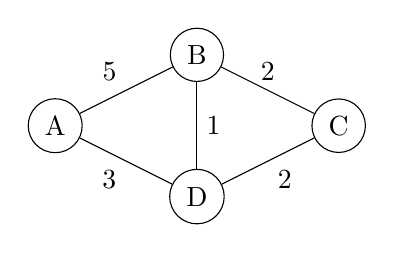
\begin{tikzpicture}[>=stealth, scale=0.9]
                \node[draw,circle] (A) at (0,0) {A};
                \node[draw,circle] (B) at (2,1) {B};
                \node[draw,circle] (C) at (4,0) {C};
                \node[draw,circle] (D) at (2,-1) {D};
                \draw (A) -- node[above left]{5} (B);
                \draw (A) -- node[below left]{3} (D);
                \draw (B) -- node[above]{2} (C);
                \draw (B) -- node[right]{1} (D);
                \draw (C) -- node[below right]{2} (D);
            \end{tikzpicture}
        \end{center}
    \end{exampleblock}
\end{frame}

\begin{frame}{OSPF --- 区域划分}
    \begin{center}
        \begin{tikzpicture}[>=stealth]
            \node[draw,circle,minimum size=1.2cm,fill=red!20] (area0) at (0,0) {Area 0\\骨干区域};
            \node[draw,circle,minimum size=1cm,fill=blue!20] (area1) at (-2.5,-2) {Area 1};
            \node[draw,circle,minimum size=1cm,fill=blue!20] (area2) at (2.5,-2) {Area 2};
            \node[draw,circle,minimum size=1cm,fill=blue!20] (area3) at (0,2) {Area 3};
            \draw (area0) -- (area1);
            \draw (area0) -- (area2);
            \draw (area0) -- (area3);
            \node[below] at (-2.5,-2.8) {普通区域};
            \node[below] at (0,-0.8) {所有区域必须与Area 0相连};
        \end{tikzpicture}
    \end{center}
    \vspace{0.3em}
    \begin{itemize}
        \item \textbf{骨干区域（Area 0）}：所有非骨干区域必须与其相连
        \item \textbf{普通区域}：通过ABR（区域边界路由器）连接骨干区域
        \item \textbf{优点}：限制LSA泛洪范围，减少路由计算量
    \end{itemize}
\end{frame}

\begin{frame}{距离向量 vs 链路状态}
    \begin{table}
        \centering
        \begin{tabular}{|c|c|c|}
            \hline
            \textbf{特性} & \textbf{距离向量（RIP）} & \textbf{链路状态（OSPF）} \\
            \hline
            交换内容 & 整张路由表 & 链路状态信息 \\
            算法 & Bellman-Ford & Dijkstra \\
            收敛速度 & 慢 & 快 \\
            跳数限制 & 15跳 & 无 \\
            更新方式 & 定期(30s) & 触发 \\
            复杂性 & 简单 & 复杂 \\
            适用规模 & 小型网络 & 大型网络 \\
            \hline
        \end{tabular}
    \end{table}
    \vspace{0.5em}
    \begin{itemize}
        \item RIP：实现简单，易出现计数到无穷问题
        \item OSPF：收敛快，适合大型网络，支持层次划分
    \end{itemize}
\end{frame}



\begin{frame}{本节总结}
    \begin{enumerate}
        \item 静态路由（手动配置）vs 动态路由（自动计算）
        \item 距离向量算法（RIP）：Bellman-Ford方程，邻居交换路由表，跳数$\le$15，慢收敛、计数到无穷
        \item 链路状态算法（OSPF）：收集全网LS，Dijkstra计算，触发更新，收敛快，区域划分
        \item BGP：自治系统间路由，路径向量算法，TCP 179
    \end{enumerate}
\end{frame}

\end{document}


\subsection{4-12 传输层概述}
\documentclass[10pt, aspectratio=169]{beamer}
\usepackage{../beamer_theme_408}
\title{408考研零基础 --- 计算机网络}
\subtitle{4-12 传输层概述}
\author{}
\date{}
\begin{document}

\begin{frame}{本节目标}
    \begin{enumerate}
        \item 理解传输层的功能：端到端通信、进程到进程
        \item 理解端口号的概念与分类
        \item 掌握UDP协议特点及首部格式
        \item 掌握TCP协议特点，对比UDP
    \end{enumerate}
\end{frame}

\begin{frame}{传输层功能}
    \begin{block}{核心职责}
        提供\textbf{端到端}的通信服务（进程到进程），是应用层与网络层之间的桥梁。
    \end{block}
    \vspace{0.3em}
    \begin{center}
        \begin{tikzpicture}[>=stealth]
            \node[draw,minimum width=2.5cm,minimum height=0.6cm,fill=blue!20] at (-2,1.5) {应用层（进程）};
            \node[draw,minimum width=2.5cm,minimum height=0.6cm,fill=blue!20] at (2,1.5) {应用层（进程）};
            \node[draw,minimum width=2.5cm,minimum height=0.6cm,fill=red!20] at (-2,0.5) {\textbf{传输层}};
            \node[draw,minimum width=2.5cm,minimum height=0.6cm,fill=red!20] at (2,0.5) {\textbf{传输层}};
            \node[draw,minimum width=2.5cm,minimum height=0.6cm,fill=green!20] at (-2,-0.5) {网络层};
            \node[draw,minimum width=2.5cm,minimum height=0.6cm,fill=green!20] at (2,-0.5) {网络层};
            \draw[<->,thick] (-2,0.5) -- node[above]{端到端连接}(2,0.5);
            \draw[<->] (-2,-0.5) -- node[below]{逐跳转发}(2,-0.5);
            \draw[<->] (-2,1.2) -- (-2,0.8);
            \draw[<->] (2,1.2) -- (2,0.8);
        \end{tikzpicture}
    \end{center}
    \vspace{0.3em}
    \begin{columns}[t]
        \column{0.48\textwidth}
        \textbf{传输层提供的服务}
        \begin{itemize}
            \item 进程到进程通信
            \item 复用与分用
            \item 差错检测
            \item 流量控制
            \item 可靠传输（TCP）
        \end{itemize}
        \column{0.48\textwidth}
        \textbf{用端口号标识进程}
        \begin{itemize}
            \item IP地址标识主机
            \item 端口号标识进程
            \item 套接字 = IP + 端口
        \end{itemize}
    \end{columns}
\end{frame}

\begin{frame}{端口号}
    \begin{block}{端口号范围}
        16位端口号，范围0 -- 65535。
    \end{block}
    \vspace{0.3em}
    \begin{columns}[t]
        \column{0.33\textwidth}
        \textbf{熟知端口(0-1023)}
        \begin{itemize}
            \item HTTP: 80
            \item FTP: 21/20
            \item DNS: 53
            \item SMTP: 25
            \item SSH: 22
            \item HTTPS: 443
        \end{itemize}
        \column{0.33\textwidth}
        \textbf{登记端口(1024-49151)}
        \begin{itemize}
            \item 需IANA登记
            \item 避免冲突
            \item 例：8080(HTTP代理)
        \end{itemize}
        \column{0.33\textwidth}
        \textbf{动态端口(49152-65535)}
        \begin{itemize}
            \item 客户端临时使用
            \item 操作系统分配
            \item 通信完成后释放
        \end{itemize}
    \end{columns}
    \vspace{0.5em}
    \begin{center}
        \begin{tikzpicture}[>=stealth]
            \draw[->] (0,0) -- (8,0) node[right]{端口号};
            \draw[red,thick] (0,0.1) -- (1.5,0.1);
            \draw[blue,thick] (1.5,0.1) -- (6,0.1);
            \draw[green,thick] (6,0.1) -- (8,0.1);
            \node[align=center,above] at (0.75,0.4) {\small 熟知\\0-1023};
            \node[align=center,above] at (3.75,0.4) {\small 登记\\1024-49151};
            \node[align=center,above] at (7,0.4) {\small 动态\\49152-65535};
        \end{tikzpicture}
    \end{center}
\end{frame}

\begin{frame}{复用与分用}
    \begin{columns}[t]
        \column{0.5\textwidth}
        \textbf{复用}
        \begin{itemize}
            \item 多个应用层进程（如浏览器、邮件、FTP）
            \item 共用同一个传输层协议
            \item 封装时加上各自端口号
        \end{itemize}
        \vspace{0.5em}
        \begin{center}
            \begin{tikzpicture}[>=stealth]
                \node[draw,minimum width=1.5cm] (p1) at (-1.2,1.5) {进程1};
                \node[draw,minimum width=1.5cm] (p2) at (0,1.5) {进程2};
                \node[draw,minimum width=1.5cm] (p3) at (1.2,1.5) {进程3};
                \node[draw,minimum width=4cm] (t) at (0,0.5) {传输层};
                \draw[->] (p1) -- (t);
                \draw[->] (p2) -- (t);
                \draw[->] (p3) -- (t);
                \draw[->] (t) -- (0,-0.5);
                \node at (0,-1) {复用};
            \end{tikzpicture}
        \end{center}
        \column{0.5\textwidth}
        \textbf{分用}
        \begin{itemize}
            \item 传输层收到数据后
            \item 根据目的端口号
            \item 分发到对应应用进程
        \end{itemize}
        \vspace{0.5em}
        \begin{center}
            \begin{tikzpicture}[>=stealth]
                \node[draw,minimum width=4cm] (t) at (0,0.5) {传输层};
                \node[draw,minimum width=1.5cm] (p1) at (-1.2,-0.5) {进程1};
                \node[draw,minimum width=1.5cm] (p2) at (0,-0.5) {进程2};
                \node[draw,minimum width=1.5cm] (p3) at (1.2,-0.5) {进程3};
                \draw[->] (t) -- (p1);
                \draw[->] (t) -- (p2);
                \draw[->] (t) -- (p3);
                \draw[->] (0,1.2) -- (t);
                \node at (0,-1.2) {分用};
            \end{tikzpicture}
        \end{center}
    \end{columns}
\end{frame}

\begin{frame}{UDP协议特点}
    \begin{block}{UDP (User Datagram Protocol)}
        用户数据报协议，提供\textbf{无连接、不可靠}的传输服务。
    \end{block}
    \vspace{0.3em}
    \begin{columns}[t]
        \column{0.5\textwidth}
        \textbf{特点}
        \begin{itemize}
            \item \textbf{无连接}：发送前不建立连接
            \item \textbf{不可靠}：不保证送达，无确认重传
            \item \textbf{面向报文}：保留报文边界
            \item \textbf{开销小}：首部仅8字节
            \item \textbf{支持广播/组播}
        \end{itemize}
        \column{0.5\textwidth}
        \textbf{适用场景}
        \begin{itemize}
            \item DNS查询
            \item 视频/音频流媒体
            \item 实时游戏
            \item DHCP
            \item SNMP
        \end{itemize}
    \end{columns}
\end{frame}

\begin{frame}{UDP首部格式}
    \begin{center}
        \begin{tikzpicture}[>=stealth]
            \draw[thick] (0,0) -- (8,0);
            \draw[thick] (0,0) -- (0,-3.5);
            \draw[thick] (8,0) -- (8,-3.5);
            \draw[thick] (0,-3.5) -- (8,-3.5);
            \draw[thick] (4,0) -- (4,-0.8);
            \draw[thick] (0,-0.8) -- (8,-0.8);
            \draw[thick] (4,-0.8) -- (4,-1.6);
            \draw[thick] (0,-1.6) -- (8,-1.6);
            \draw[thick] (4,-1.6) -- (4,-2.4);
            \draw[thick] (0,-2.4) -- (8,-2.4);
            \node at (2,-0.4) {源端口(16位)};
            \node at (6,-0.4) {目的端口(16位)};
            \node at (2,-1.2) {UDP长度(16位)};
            \node at (6,-1.2) {UDP校验和(16位)};
            \node[draw,minimum width=8cm,minimum height=0.8cm,fill=gray!20] at (4,-2.8) {数据部分};
            \node[above] at (4,0.3) {\textbf{UDP首部（8字节）}};
        \end{tikzpicture}
    \end{center}
    \vspace{0.3em}
    \begin{itemize}
        \item 源端口：发送方端口（可选，不需应答时填0）
        \item 目的端口：接收方端口
        \item UDP长度：首部+数据的总长度（字节）
        \item 校验和：检测传输差错（可选，IPv4中可置0）
    \end{itemize}
\end{frame}

\begin{frame}{TCP协议特点}
    \begin{block}{TCP (Transmission Control Protocol)}
        传输控制协议，提供\textbf{面向连接、可靠}的传输服务。
    \end{block}
    \vspace{0.3em}
    \begin{columns}[t]
        \column{0.5\textwidth}
        \textbf{特点}
        \begin{itemize}
            \item \textbf{面向连接}：三次握手建立，四次挥手释放
            \item \textbf{可靠传输}：确认+重传
            \item \textbf{面向字节流}：不保留报文边界
            \item \textbf{全双工通信}
            \item \textbf{流量控制}（滑动窗口）
            \item \textbf{拥塞控制}
        \end{itemize}
        \column{0.5\textwidth}
        \textbf{适用场景}
        \begin{itemize}
            \item 网页浏览（HTTP）
            \item 文件传输（FTP）
            \item 电子邮件（SMTP）
            \item 远程登录（SSH）
            \item 数据库连接
        \end{itemize}
    \end{columns}
\end{frame}

\begin{frame}{TCP vs UDP对比}
    \begin{table}
        \centering
        \begin{tabular}{|c|c|c|}
            \hline
            \textbf{特性} & \textbf{TCP} & \textbf{UDP} \\
            \hline
            连接 & 面向连接 & 无连接 \\
            可靠性 & 可靠（确认重传） & 不可靠（尽力而为） \\
            数据边界 & 字节流 & 报文边界 \\
            首部大小 & 20字节 & 8字节 \\
            速度 & 慢 & 快 \\
            全双工 & 是 & 半双工（单工） \\
            流量/拥塞控制 & 支持 & 不支持 \\
            广播/组播 & 不支持 & 支持 \\
            典型应用 & HTTP/FTP/SMTP & DNS/视频/DHCP \\
            \hline
        \end{tabular}
    \end{table}
    \vspace{0.5em}
    \begin{exampleblock}{选择原则}
        \begin{itemize}
            \item 需要可靠传输 $\rightarrow$ TCP
            \item 实时性要求高、允许丢包 $\rightarrow$ UDP
        \end{itemize}
    \end{exampleblock}
\end{frame}

\begin{frame}{本节总结}
    \begin{enumerate}
        \item 传输层功能：端到端、进程到进程（端口号标识），复用与分用
        \item 端口号：熟知0-1023、登记1024-49151、动态49152-65535
        \item UDP：无连接、不可靠、面向报文、首部8字节
        \item TCP：面向连接、可靠、面向字节流、全双工、首部20字节
    \end{enumerate}
\end{frame}
\end{document}


\subsection{4-13 TCP协议}
\documentclass[10pt, aspectratio=169]{beamer}
\usepackage{../beamer_theme_408}
\title{408考研零基础 --- 计算机网络}
\subtitle{4-13 TCP协议}
\author{}
\date{}
\begin{document}

\begin{frame}{本节目标}
    \begin{enumerate}
        \item 掌握TCP报文段首部格式及各字段含义
        \item 理解三次握手建立连接和四次挥手释放连接的过程
        \item 理解TCP的可靠传输、流量控制和拥塞控制机制
    \end{enumerate}
\end{frame}

\begin{frame}{TCP报文段首部}
    \begin{center}
        \begin{tikzpicture}[>=stealth, scale=0.65, every node/.style={scale=0.65}]
            \draw[thick] (0,0) -- (12,0);
            \draw[thick] (0,0) -- (0,-7);
            \draw[thick] (12,0) -- (12,-7);
            \draw[thick] (0,-7) -- (12,-7);
            \foreach \x in {2,4,6,8,10} {
                \draw[thick] (\x,0) -- (\x,-7);
            }
            \foreach \y in {0.7,1.4,2.1,2.8,3.5,4.2,4.9,5.6,6.3} {
                \draw[thick] (0,-\y) -- (12,-\y);
            }
            \node at (1,-0.35) {源端口(16)};
            \node at (7,-0.35) {目的端口(16)};
            \node at (3,-1.05) {序号(32)};
            \node at (3,-1.75) {确认号(32)};
            \node at (1,-2.45) {数据偏移(4)};
            \node at (2.5,-2.45) {保留(6)};
            \node at (5,-2.45) {标志位(6)};
            \node at (7,-2.45) {窗口(16)};
            \node at (3,-3.15) {校验和(16)};
            \node at (9,-3.15) {紧急指针(16)};
            \node[draw,minimum width=12cm,minimum height=2.8cm,fill=gray!20] at (6,-5.2) {选项（可变长度，填充至32位对齐）};
            \node[draw,minimum width=12cm,minimum height=0.5cm,fill=blue!20] at (6,-7.7) {数据部分};
            \node[above] at (6,0.3) {\textbf{TCP首部（20字节固定 + 选项）}};
            \node[align=left,below] at (0,0.3) {0};
            \node[align=left,below] at (2,0.3) {4};
            \node[align=left,below] at (4,0.3) {8};
            \node[align=left,below] at (6,0.3) {12};
            \node[align=left,below] at (8,0.3) {16};
            \node[align=left,below] at (10,0.3) {20};
            \node[align=left,below] at (12,0.3) {24};
        \end{tikzpicture}
    \end{center}
\end{frame}

\begin{frame}{标志位详解}
    \begin{block}{6个标志位（每位置1有效）}
        \begin{description}
            \item[URG] 紧急指针标志，紧急数据优先处理
            \item[ACK] 确认号有效（建立连接后通常置1）
            \item[PSH] 推送，接收方应尽快交付应用层
            \item[RST] 重置连接（异常断开）
            \item[SYN] 同步序号，用于建立连接
            \item[FIN] 释放连接
        \end{description}
    \end{block}
    \vspace{0.5em}
    \begin{exampleblock}{关键字段}
        \begin{itemize}
            \item \textbf{序号}：本报文段数据第一个字节的序号
            \item \textbf{确认号}：期望收到对方下一个数据字节的序号
            \item \textbf{窗口}：接收方通告的剩余缓冲区大小（rwnd）
        \end{itemize}
    \end{exampleblock}
\end{frame}

\begin{frame}{三次握手 --- 建立连接}
    \begin{center}
        \begin{tikzpicture}[>=stealth, node distance=1.2cm]
            \node (A) {\textbf{客户端}};
            \node[right=5cm of A] (B) {\textbf{服务器}};
            
            \draw[->,thick] (A) to[out=0,in=180] node[above]{\small SYN=1, seq=x} (B);
            \draw[->,thick] (B) to[out=180,in=0] node[below]{\small SYN=1, ACK=1, seq=y, ack=x+1} (A);
            \draw[->,thick] (A) to[out=0,in=180] node[above]{\small ACK=1, seq=x+1, ack=y+1} (B);
            
            \node[left=0.3cm of A] (t1) {1.};
            \node[left=0.3cm of A] (t2) at (0,-1.2) {2.};
            \node[left=0.3cm of A] (t3) at (0,-2.4) {3.};
        \end{tikzpicture}
    \end{center}
    \vspace{0.3em}
    \begin{enumerate}
        \item 客户端发送SYN报文（seq=x），进入SYN\_SENT状态
        \item 服务器回复SYN+ACK（seq=y, ack=x+1），进入SYN\_RCVD状态
        \item 客户端发送ACK（seq=x+1, ack=y+1），双方进入ESTABLISHED状态
    \end{enumerate}
\end{frame}

\begin{frame}{为什么需要三次握手？}
    \begin{block}{核心原因}
        防止已失效的连接请求到达服务器，造成资源浪费。
    \end{block}
    \vspace{0.3em}
    \begin{exampleblock}{场景说明}
        \begin{enumerate}
            \item 客户端发送连接请求SYN（第一次）
            \item 该请求在网络中延迟，客户端未收到ACK
            \item 客户端重传SYN并成功建立连接，传输数据后释放
            \item 延迟的旧SYN到达服务器，服务器误以为新请求
            \item 若只有两次握手，服务器会建立空连接并等待数据
            \item 三次握手：服务器回复SYN+ACK，客户端不回应（因无此请求），服务器超时释放
        \end{enumerate}
    \end{exampleblock}
    \vspace{0.3em}
    \begin{alertblock}{结论}
        第三次握手用于确认客户端确实有建立连接的意愿。
    \end{alertblock}
\end{frame}

\begin{frame}{四次挥手 --- 释放连接}
    \begin{center}
        \begin{tikzpicture}[>=stealth, node distance=1.2cm]
            \node (A) {\textbf{客户端}};
            \node[right=5cm of A] (B) {\textbf{服务器}};
            
            \draw[->,thick] (A) to[out=0,in=180] node[above]{\small FIN=1, seq=u} (B);
            \node[right=0.2cm of B] (s1) {CLOSE\_WAIT};
            \draw[->,thick] (B) to[out=180,in=0] node[below]{\small ACK=1, seq=v, ack=u+1} (A);
            \node[left=0.2cm of A] (s2) {FIN\_WAIT\_2};
            \draw[->,thick] (B) to[out=180,in=0] node[below]{\small FIN=1, ACK=1, seq=w, ack=u+1} (A);
            \draw[->,thick] (A) to[out=0,in=180] node[above]{\small ACK=1, seq=u+1, ack=w+1} (B);
            \node[right=0.2cm of B] (s3) {CLOSED};
            \node[left=0.2cm of A] (s4) {TIME\_WAIT};
        \end{tikzpicture}
    \end{center}
    \vspace{0.3em}
    \begin{enumerate}
        \item 客户端发送FIN，进入FIN\_WAIT\_1
        \item 服务器回复ACK，进入CLOSE\_WAIT（客户端FIN\_WAIT\_2）
        \item 服务器发送FIN，进入LAST\_ACK
        \item 客户端回复ACK，进入TIME\_WAIT（2MSL后关闭）
    \end{enumerate}
\end{frame}

\begin{frame}{TIME\_WAIT 2MSL}
    \begin{block}{为什么TIME\_WAIT需要等待2MSL？}
        MSL（Maximum Segment Lifetime）：报文段最大生存时间。
    \end{block}
    \vspace{0.3em}
    \begin{enumerate}
        \item \textbf{确保最后一个ACK到达}
        \begin{itemize}
            \item 若ACK丢失，服务器超时重传FIN
            \item 客户端在2MSL内能收到重传的FIN并重新ACK
        \end{itemize}
        \item \textbf{使旧连接报文消失}
        \begin{itemize}
            \item 2MSL足够让本连接所有旧报文在网络中消失
            \item 防止影响新连接（相同IP和端口）
        \end{itemize}
    \end{enumerate}
    \vspace{0.5em}
    \begin{center}
        \begin{tikzpicture}[>=stealth]
            \draw[->] (0,0) -- (6,0);
            \draw[red,thick] (0,0.1) -- node[above]{TIME\_WAIT (2MSL)} (4,0.1);
            \node at (2,0.4) {\small 等待期间：端口被占用，不能使用};
            \draw[->,dashed] (0.3,0.5) -- (1.5,0.5);
            \node[above] at (0.9,0.8) {若FIN重传，可重新ACK};
        \end{tikzpicture}
    \end{center}
\end{frame}

\begin{frame}{可靠传输机制}
    \begin{block}{TCP如何实现可靠传输？}
        序号 + 确认 + 超时重传
    \end{block}
    \vspace{0.3em}
    \begin{columns}[t]
        \column{0.33\textwidth}
        \textbf{序号}
        \begin{itemize}
            \item 每个字节一个序号
            \item 首次序号ISN随机选择
            \item 确保数据按序重组
        \end{itemize}
        \column{0.33\textwidth}
        \textbf{确认}
        \begin{itemize}
            \item 累积确认
            \item 确认号 = 期望下个字节序号
            \item 接收方也可捎带确认
        \end{itemize}
        \column{0.33\textwidth}
        \textbf{超时重传}
        \begin{itemize}
            \item 发送时启动计时器
            \item RTO动态计算
            \item 基于RTT估算
        \end{itemize}
    \end{columns}
    \vspace{0.5em}
    \begin{exampleblock}{重传策略}
        \begin{itemize}
            \item 超时未收到ACK $\rightarrow$ 重传
            \item 收到3个冗余ACK $\rightarrow$ 快重传
        \end{itemize}
    \end{exampleblock}
\end{frame}

\begin{frame}{流量控制}
    \begin{block}{滑动窗口机制}
        接收方通过\textbf{rwnd（接收窗口）}告知发送方自己的剩余缓冲区大小，发送方据此调整发送速率。
    \end{block}
    \vspace{0.3em}
    \begin{center}
        \begin{tikzpicture}[>=stealth]
            \node[draw,minimum width=8cm,minimum height=0.6cm] (buf) at (0,0) {};
            \node[above] at (-3,0.3) {发送缓冲区};
            \fill[blue!20] (-3.8,0) rectangle (-0.5,0.6);
            \fill[green!20] (-0.5,0) rectangle (2.5,0.6);
            \fill[gray!20] (2.5,0) rectangle (4.2,0.6);
            \node[above] at (-2.15,0.8) {已确认};
            \node[above] at (1,0.8) {已发送待确认};
            \node[above] at (3.35,0.8) {未发送};
            \draw[decorate,decoration={brace,amplitude=5pt}] (2.5,0.6) -- (4.2,0.6);
            \node[above] at (3.35,1.2) {窗口大小 = rwnd};
        \end{tikzpicture}
    \end{center}
    \vspace{0.3em}
    \begin{columns}[t]
        \column{0.48\textwidth}
        \textbf{过程}
        \begin{enumerate}
            \item 接收方在ACK中通告rwnd
            \item 发送方窗口 $\le$ rwnd
            \item rwnd = 0时，发送方停止发送
        \end{enumerate}
        \column{0.48\textwidth}
        \textbf{持续计时器}
        \begin{itemize}
            \item 防止rwnd=0时死锁
            \item 发送方定期发送探测段
            \item 了解接收方窗口是否变化
        \end{itemize}
    \end{columns}
\end{frame}

\begin{frame}{拥塞控制}
    \begin{block}{核心目标}
        防止过多数据注入网络，避免网络过载。发送方维护\textbf{拥塞窗口cwnd}。
        \[
        \text{实际发送窗口} = \min(\text{cwnd}, \text{rwnd})
        \]
    \end{block}
    \vspace{0.3em}
    \begin{center}
        \begin{tikzpicture}[>=stealth]
            \draw[->] (0,0) -- (8,0) node[right]{时间};
            \draw[->] (0,0) -- (0,4) node[above]{cwnd};
            
            \draw[blue,thick] plot coordinates {(0,1) (1,2) (2,4) (3,4) (4,5) (5,6) (6,7) (7,8)};
            \draw[red,dashed] (1,3) -- (7,3) node[right]{ssthresh};
            
            \node at (0.5,1.3) {\small 慢开始};
            \node at (2.5,4.5) {\small 拥塞避免};
            \draw[decorate,decoration={zigzag}] (0.5,0.5) -- (0.5,1);
            
            \node[below] at (2,0) {阈值};
        \end{tikzpicture}
    \end{center}
\end{frame}

\begin{frame}{慢开始与拥塞避免}
    \begin{columns}[t]
        \column{0.5\textwidth}
        \textbf{慢开始}
        \begin{itemize}
            \item cwnd初始值为1MSS
            \item 每收到一个ACK，cwnd+1
            \item 每经过一个RTT，cwnd $\times 2$
            \item \textbf{指数增长}
            \item 直到ssthresh（慢开始阈值）
        \end{itemize}
        \column{0.5\textwidth}
        \textbf{拥塞避免}
        \begin{itemize}
            \item cwnd $\ge$ ssthresh进入此阶段
            \item 每经过一个RTT，cwnd+1
            \item \textbf{线性增长}
            \item 直到发生丢包（超时或3冗余ACK）
        \end{itemize}
    \end{columns}
    \vspace{0.5em}
    \begin{exampleblock}{拥塞发生时的处理}
        \begin{itemize}
            \item \textbf{超时}：ssthresh = cwnd/2，cwnd = 1，重新慢开始
            \item \textbf{3冗余ACK}：ssthresh = cwnd/2，cwnd = ssthresh，快恢复
        \end{itemize}
    \end{exampleblock}
\end{frame}

\begin{frame}{快重传与快恢复}
    \begin{columns}[t]
        \column{0.5\textwidth}
        \textbf{快重传}
        \begin{itemize}
            \item 接收方收到乱序段时立即发送\textbf{冗余ACK}
            \item 发送方收到\textbf{3个冗余ACK}立即重传
            \item 不等超时
            \item 提高重传效率
        \end{itemize}
        \vspace{0.3em}
        \begin{center}
            \begin{tikzpicture}[>=stealth, scale=0.6]
                \draw[->] (0,0) -- (4,0);
                \foreach \x/\l in {0/1,1/2,2/3,3/4} {
                    \fill[blue!20] (\x*0.8,0) rectangle (\x*0.8+0.4,0.3);
                    \node at (\x*0.8+0.2,-0.2) {\l};
                }
                \fill[red!30] (0.8*2,0.3) -- (0.8*2+0.4,0.3) -- (0.8*2+0.2,0.6) -- cycle;
                \node at (1.6,-0.5) {丢包};
                \node at (3.2,-0.5) {$\leftarrow$ 3冗余ACK触发重传};
            \end{tikzpicture}
        \end{center}
        \column{0.5\textwidth}
        \textbf{快恢复}
        \begin{itemize}
            \item 收到3冗余ACK时执行
            \item ssthresh = cwnd / 2
            \item cwnd = ssthresh
            \item 从\textbf{拥塞避免}阶段开始
            \item 不回到慢开始
        \end{itemize}
    \end{columns}
    \vspace{0.5em}
    \begin{block}{完整拥塞控制流程}
        慢开始（指数） $\rightarrow$ 拥塞避免（线性） $\rightarrow$ 丢包$\rightarrow$ 快重传+快恢复（或超时重回慢开始）
    \end{block}
\end{frame}

\begin{frame}{拥塞控制状态图}
    \begin{center}
        \begin{tikzpicture}[>=stealth, node distance=1.2cm]
            \node[draw,minimum width=2cm,minimum height=0.8cm,fill=green!20] (ss) {慢开始};
            \node[draw,minimum width=2cm,minimum height=0.8cm,fill=blue!20,right=1.5cm of ss] (ca) {拥塞避免};
            \node[draw,minimum width=2cm,minimum height=0.8cm,fill=red!20,below=1cm of ca] (fr) {快恢复};
            
            \draw[->] (ss) -- node[above]{cwnd $\ge$ ssthresh} (ca);
            \draw[->] (ca) to[out=180,in=0] node[above,yshift=0.3cm]{超时：ssthresh=cwnd/2, cwnd=1} (ss);
            \draw[->] (ca) -- node[right]{3冗余ACK：ssthresh=cwnd/2, cwnd=ssthresh} (fr);
            \draw[->] (fr) to[out=0,in=0] node[left]{新ACK} (ca);
            \draw[->] (fr) to[out=180,in=270] node[below]{超时} (ss);
        \end{tikzpicture}
    \end{center}
\end{frame}

\begin{frame}{本节总结}
    \begin{enumerate}
        \item TCP报文段首部：20字节固定，含源/目的端口、序号、确认号、标志位、窗口等
        \item 三次握手（SYN$\to$SYN+ACK$\to$ACK）防止失效连接请求；四次挥手（FIN$\to$ACK$\to$FIN$\to$ACK），TIME\_WAIT 2MSL
        \item 可靠传输：序号+确认+超时重传；流量控制：滑动窗口rwnd；拥塞控制：慢开始+拥塞避免+快重传+快恢复
    \end{enumerate}
\end{frame}
\end{document}


\subsection{4-14 应用层协议}
\documentclass[10pt, aspectratio=169]{beamer}
\usepackage{../beamer_theme_408}
\title{408考研零基础 --- 计算机网络}
\subtitle{4-14 应用层协议}
\author{}
\date{}
\begin{document}

\begin{frame}{本节目标}
    \begin{enumerate}
        \item 掌握DNS域名系统的层次结构和查询方式
        \item 理解HTTP协议的特点、请求方法和状态码
        \item 理解FTP、SMTP、POP3、IMAP等应用层协议
    \end{enumerate}
\end{frame}

\begin{frame}{应用层概述}
    \begin{block}{应用层的作用}
        为应用程序提供网络通信服务，是用户与网络的接口。
    \end{block}
    \vspace{0.3em}
    \begin{center}
        \begin{tikzpicture}[>=stealth]
            \node[draw,minimum width=10cm,minimum height=0.6cm,fill=blue!20] at (0,0) {\textbf{应用层协议}};
            \foreach \x/\name in {-4.2/DNS, -2.4/HTTP, -0.6/FTP, 1.2/SMTP, 3/POP3, 4.6/Telnet} {
                \node at (\x,-0.8) {\name};
            }
            \foreach \x/\name in {-4.2/DNS, -2.4/HTTP, -0.6/FTP, 1.2/SMTP, 3/POP3, 4.6/Telnet} {
                \draw[->] (\x,-0.5) -- (\x,-0.2);
            }
            \node[draw,minimum width=10cm,minimum height=0.6cm,fill=red!20] at (0,-1.6) {传输层（TCP/UDP）};
        \end{tikzpicture}
    \end{center}
    \vspace{0.3em}
    \begin{itemize}
        \item 应用层协议定义了应用进程间通信的规则
        \item 每个应用层协议通常对应一个标准端口号
        \item C/S模式：客户端主动请求，服务器被动响应
    \end{itemize}
\end{frame}

\begin{frame}{DNS域名系统}
    \begin{block}{功能}
        将人类易记的域名（如 www.example.com）解析为IP地址。
    \end{block}
    \vspace{0.3em}
    \begin{center}
        \begin{tikzpicture}[>=stealth]
            \node (root) at (0,2) {根域名服务器};
            \node (top) at (-2.5,0.8) {.com顶级域};
            \node (top2) at (2.5,0.8) {.cn顶级域};
            \node (sec) at (-2.5,-0.8) {example.com};
            \node (host) at (-2.5,-2) {www.example.com};
            \draw (root) -- (top);
            \draw (root) -- (top2);
            \draw (top) -- (sec);
            \draw (sec) -- (host);
            \node[right] at (0,2.4) {根域（.）};
            \node[right] at (-2.5,1.2) {顶级域（TLD）};
            \node[right] at (-2.5,-0.4) {二级域};
            \node[right] at (-2.5,-1.6) {子域};
        \end{tikzpicture}
    \end{center}
    \vspace{0.3em}
    \begin{itemize}
        \item 层次树形结构：根域 $\rightarrow$ 顶级域 $\rightarrow$ 二级域 $\rightarrow$ 子域
        \item 域名服务器层次对应域名层次
    \end{itemize}
\end{frame}

\begin{frame}{DNS查询方式}
    \begin{columns}[t]
        \column{0.48\textwidth}
        \textbf{递归查询}
        \begin{enumerate}
            \item 主机问本地DNS服务器
            \item 本地DNS替主机逐级查询
            \item 最终返回结果给主机
        \end{enumerate}
        \vspace{0.3em}
        \begin{center}
            \begin{tikzpicture}[>=stealth, scale=0.6]
                \node (h) {主机};
                \node[right=1.2cm of h] (l) {本地DNS};
                \node[right=1.2cm of l] (r) {根DNS};
                \node[right=1.2cm of r] (t) {顶级DNS};
                \draw[->] (h) -- (l);
                \draw[->] (l) -- (r);
                \draw[->] (r) -- (t);
                \draw[->] (t) -- (r);
                \draw[->] (r) -- (l);
                \draw[->] (l) -- (h);
            \end{tikzpicture}
        \end{center}
        \column{0.48\textwidth}
        \textbf{迭代查询}
        \begin{enumerate}
            \item 主机问本地DNS服务器
            \item 本地DNS依次问各级DNS
            \item 各级DNS告诉"去问谁"
            \item 最后回复结果
        \end{enumerate}
        \vspace{0.3em}
        \begin{center}
            \begin{tikzpicture}[>=stealth, scale=0.6]
                \node (h) {主机};
                \node[right=1.2cm of h] (l) {本地DNS};
                \node[right=1.2cm of l] (r) {根DNS};
                \node[above right=0.5cm and 0.5cm of r] (t) {顶级DNS};
                \draw[->] (h) -- (l);
                \draw[->] (l) -- (r);
                \draw[->,dashed] (r) -- (l);
                \draw[->] (l) -- (t);
                \draw[->,dashed] (t) -- (l);
                \draw[->] (l) -- (h);
            \end{tikzpicture}
        \end{center}
    \end{columns}
    \vspace{0.5em}
    \begin{itemize}
        \item 递归：查询负担在DNS服务器，结果直接返回
        \item 迭代："你问他，他再告诉你"依次询问
    \end{itemize}
\end{frame}

\begin{frame}{HTTP协议}
    \begin{block}{HTTP (HyperText Transfer Protocol)}
        超文本传输协议，基于C/S模式，默认端口80。
    \end{block}
    \vspace{0.3em}
    \begin{center}
        \begin{tikzpicture}[>=stealth]
            \node[draw,minimum width=2cm,minimum height=1cm,fill=blue!20] (c) {客户端};
            \node[draw,minimum width=2cm,minimum height=1cm,fill=green!20,right=3cm of c] (s) {服务器};
            \draw[<->,thick] (c) -- node[above]{HTTP请求/响应} (s);
            \node at (0,-0.8) {浏览器};
            \node at (5,-0.8) {Web服务器};
        \end{tikzpicture}
    \end{center}
    \vspace{0.5em}
    \begin{columns}[t]
        \column{0.48\textwidth}
        \textbf{持久连接}
        \begin{itemize}
            \item Keep-Alive
            \item 多个请求共用一个TCP
            \item 减少连接开销
            \item HTTP/1.1默认
        \end{itemize}
        \column{0.48\textwidth}
        \textbf{非持久连接}
        \begin{itemize}
            \item 每个请求新建TCP
            \item 开销大，效率低
            \item HTTP/1.0默认
        \end{itemize}
    \end{columns}
\end{frame}

\begin{frame}{HTTP请求方法与状态码}
    \begin{columns}[t]
        \column{0.48\textwidth}
        \textbf{常见请求方法}
        \begin{itemize}
            \item \textbf{GET}：请求资源
            \item \textbf{POST}：提交数据
            \item \textbf{HEAD}：获取响应头
            \item \textbf{PUT}：上传资源
            \item \textbf{DELETE}：删除资源
            \item \textbf{OPTIONS}：查询支持方法
        \end{itemize}
        \column{0.48\textwidth}
        \textbf{状态码分类}
        \begin{itemize}
            \item \textbf{1xx}：信息（100 Continue）
            \item \textbf{2xx}：成功（200 OK）
            \item \textbf{3xx}：重定向
            \begin{itemize}
                \item 301 永久重定向
                \item 302 临时重定向
            \end{itemize}
            \item \textbf{4xx}：客户端错误
            \begin{itemize}
                \item 403 Forbidden
                \item \textbf{404 Not Found}
            \end{itemize}
            \item \textbf{5xx}：服务器错误（500）
        \end{itemize}
    \end{columns}
\end{frame}

\begin{frame}{FTP文件传输协议}
    \begin{block}{FTP (File Transfer Protocol)}
        用于文件的上传和下载，默认端口21（控制连接）+ 20（数据连接）。
    \end{block}
    \vspace{0.3em}
    \begin{center}
        \begin{tikzpicture}[>=stealth]
            \node[draw,minimum width=2cm,minimum height=1cm,fill=blue!20] (c) {FTP客户端};
            \node[draw,minimum width=2cm,minimum height=1cm,fill=green!20,right=3cm of c] (s) {FTP服务器};
            \draw[->,thick] (c) -- node[above]{控制连接(21)}(s);
            \draw[<->,thick] (c) to[out=-30,in=210] node[below]{数据连接(20)}(s);
        \end{tikzpicture}
    \end{center}
    \vspace{0.3em}
    \begin{columns}[t]
        \column{0.48\textwidth}
        \textbf{主动模式}
        \begin{itemize}
            \item 客户端随机端口N
            \item 服务器用20连接客户端N+1
            \item 服务器主动连接客户端
        \end{itemize}
        \column{0.48\textwidth}
        \textbf{被动模式}
        \begin{itemize}
            \item 客户端发PASV命令
            \item 服务器开放随机端口
            \item 客户端主动连接服务器
            \item 可穿透防火墙
        \end{itemize}
    \end{columns}
    \vspace{0.3em}
    \begin{alertblock}{特点}
        \textbf{带外控制}：控制连接和数据连接分离（FTP独有）。
    \end{alertblock}
\end{frame}

\begin{frame}{电子邮件协议}
    \begin{block}{电子邮件系统组成}
        用户代理 + 邮件服务器 + 邮件协议
    \end{block}
    \vspace{0.3em}
    \begin{center}
        \begin{tikzpicture}[>=stealth]
            \node (c1) {发件人};
            \node[right=1.5cm of c1] (s1) {发送方邮件服务器};
            \node[right=1.5cm of s1] (s2) {接收方邮件服务器};
            \node[right=1.5cm of s2] (c2) {收件人};
            \draw[->] (c1) -- node[above]{SMTP} (s1);
            \draw[->] (s1) -- node[above]{SMTP} (s2);
            \draw[->] (s2) -- node[above]{POP3/IMAP} (c2);
        \end{tikzpicture}
    \end{center}
    \vspace{0.5em}
    \begin{columns}[t]
        \column{0.33\textwidth}
        \textbf{SMTP}
        \begin{itemize}
            \item 发送邮件
            \item TCP 25
            \item 推协议
        \end{itemize}
        \column{0.33\textwidth}
        \textbf{POP3}
        \begin{itemize}
            \item 接收邮件
            \item TCP 110
            \item 下载后可选删除
        \end{itemize}
        \column{0.33\textwidth}
        \textbf{IMAP}
        \begin{itemize}
            \item 接收邮件
            \item TCP 143
            \item 服务器管理邮件
            \item 支持多设备同步
        \end{itemize}
    \end{columns}
\end{frame}

\begin{frame}{应用层协议总结}
    \begin{table}
        \centering
        \begin{tabular}{|c|c|c|c|}
            \hline
            \textbf{协议} & \textbf{功能} & \textbf{端口} & \textbf{传输层} \\
            \hline
            DNS & 域名$\rightarrow$IP & 53 & UDP/TCP \\
            HTTP & 超文本传输 & 80 & TCP \\
            HTTPS & 加密HTTP & 443 & TCP \\
            FTP & 文件传输 & 21/20 & TCP \\
            SMTP & 邮件发送 & 25 & TCP \\
            POP3 & 邮件接收 & 110 & TCP \\
            IMAP & 邮件接收(高级) & 143 & TCP \\
            Telnet & 远程登录 & 23 & TCP \\
            SSH & 安全远程登录 & 22 & TCP \\
            DHCP & 动态IP配置 & 67/68 & UDP \\
            \hline
        \end{tabular}
    \end{table}
    \vspace{0.5em}
    \begin{exampleblock}{记忆技巧}
        \begin{itemize}
            \item TCP：需要可靠传输的应用（HTTP/FTP/Email/Telnet）
            \item UDP：简单查询或实时应用（DNS/DHCP）
        \end{itemize}
    \end{exampleblock}
\end{frame}

\begin{frame}{模块4 知识体系总览}
    \begin{center}
        \begin{tikzpicture}[>=stealth]
            \node[draw,fill=red!20,minimum width=6cm,minimum height=0.8cm] at (0,2.5) {\textbf{计算机网络}};
            \node[draw,fill=blue!10,minimum width=2.8cm,minimum height=0.6cm] at (-3,1.2) {应用层};
            \node[draw,fill=blue!10,minimum width=2.8cm,minimum height=0.6cm] at (0,1.2) {传输层};
            \node[draw,fill=blue!10,minimum width=2.8cm,minimum height=0.6cm] at (3,1.2) {网络层};
            \node[draw,fill=green!10,minimum width=2.8cm,minimum height=0.6cm] at (-1.5,0) {数据链路层};
            \node[draw,fill=green!10,minimum width=2.8cm,minimum height=0.6cm] at (1.5,0) {物理层};
            \draw (2.5,2.5) -- (3,2.5);
            \draw (0,2.5) -- (0,1.8);
            \draw (-3,2.5) -- (-3,1.8);
            \draw (-3,0.9) -- (-1.5,0.6);
            \draw (3,0.9) -- (1.5,0.6);
            \node[below] at (0,-0.5) {4-8 流量控制 \quad 4-9 介质访问控制};
            \node[below] at (0,-1.0) {4-10 网络层与IP \quad 4-11 路由算法};
            \node[below] at (0,-1.5) {4-12 传输层 \quad 4-13 TCP};
            \node[below] at (0,-2.0) {4-14 应用层协议};
        \end{tikzpicture}
    \end{center}
\end{frame}

\begin{frame}{本节总结}
    \begin{enumerate}
        \item DNS：层次树形命名，递归查询和迭代查询
        \item HTTP：C/S模式，持久/非持久连接，GET/POST等方法，1xx-5xx状态码
        \item FTP：21控制+20数据（带外），主动/被动模式
        \item SMTP（发送25）、POP3（接收110）、IMAP（接收143）
    \end{enumerate}
    \vspace{1em}
    \begin{center}
        \textcolor{blue}{\textbf{恭喜完成模块4全部内容！建议系统复习，融会贯通。}}
    \end{center}
\end{frame}
\end{document}


\end{document}